% Options for packages loaded elsewhere
\PassOptionsToPackage{unicode}{hyperref}
\PassOptionsToPackage{hyphens}{url}
%
\documentclass[
]{book}
\usepackage{amsmath,amssymb}
\usepackage{iftex}
\ifPDFTeX
  \usepackage[T1]{fontenc}
  \usepackage[utf8]{inputenc}
  \usepackage{textcomp} % provide euro and other symbols
\else % if luatex or xetex
  \usepackage{unicode-math} % this also loads fontspec
  \defaultfontfeatures{Scale=MatchLowercase}
  \defaultfontfeatures[\rmfamily]{Ligatures=TeX,Scale=1}
\fi
\usepackage{lmodern}
\ifPDFTeX\else
  % xetex/luatex font selection
\fi
% Use upquote if available, for straight quotes in verbatim environments
\IfFileExists{upquote.sty}{\usepackage{upquote}}{}
\IfFileExists{microtype.sty}{% use microtype if available
  \usepackage[]{microtype}
  \UseMicrotypeSet[protrusion]{basicmath} % disable protrusion for tt fonts
}{}
\makeatletter
\@ifundefined{KOMAClassName}{% if non-KOMA class
  \IfFileExists{parskip.sty}{%
    \usepackage{parskip}
  }{% else
    \setlength{\parindent}{0pt}
    \setlength{\parskip}{6pt plus 2pt minus 1pt}}
}{% if KOMA class
  \KOMAoptions{parskip=half}}
\makeatother
\usepackage{xcolor}
\usepackage{color}
\usepackage{fancyvrb}
\newcommand{\VerbBar}{|}
\newcommand{\VERB}{\Verb[commandchars=\\\{\}]}
\DefineVerbatimEnvironment{Highlighting}{Verbatim}{commandchars=\\\{\}}
% Add ',fontsize=\small' for more characters per line
\usepackage{framed}
\definecolor{shadecolor}{RGB}{248,248,248}
\newenvironment{Shaded}{\begin{snugshade}}{\end{snugshade}}
\newcommand{\AlertTok}[1]{\textcolor[rgb]{0.94,0.16,0.16}{#1}}
\newcommand{\AnnotationTok}[1]{\textcolor[rgb]{0.56,0.35,0.01}{\textbf{\textit{#1}}}}
\newcommand{\AttributeTok}[1]{\textcolor[rgb]{0.13,0.29,0.53}{#1}}
\newcommand{\BaseNTok}[1]{\textcolor[rgb]{0.00,0.00,0.81}{#1}}
\newcommand{\BuiltInTok}[1]{#1}
\newcommand{\CharTok}[1]{\textcolor[rgb]{0.31,0.60,0.02}{#1}}
\newcommand{\CommentTok}[1]{\textcolor[rgb]{0.56,0.35,0.01}{\textit{#1}}}
\newcommand{\CommentVarTok}[1]{\textcolor[rgb]{0.56,0.35,0.01}{\textbf{\textit{#1}}}}
\newcommand{\ConstantTok}[1]{\textcolor[rgb]{0.56,0.35,0.01}{#1}}
\newcommand{\ControlFlowTok}[1]{\textcolor[rgb]{0.13,0.29,0.53}{\textbf{#1}}}
\newcommand{\DataTypeTok}[1]{\textcolor[rgb]{0.13,0.29,0.53}{#1}}
\newcommand{\DecValTok}[1]{\textcolor[rgb]{0.00,0.00,0.81}{#1}}
\newcommand{\DocumentationTok}[1]{\textcolor[rgb]{0.56,0.35,0.01}{\textbf{\textit{#1}}}}
\newcommand{\ErrorTok}[1]{\textcolor[rgb]{0.64,0.00,0.00}{\textbf{#1}}}
\newcommand{\ExtensionTok}[1]{#1}
\newcommand{\FloatTok}[1]{\textcolor[rgb]{0.00,0.00,0.81}{#1}}
\newcommand{\FunctionTok}[1]{\textcolor[rgb]{0.13,0.29,0.53}{\textbf{#1}}}
\newcommand{\ImportTok}[1]{#1}
\newcommand{\InformationTok}[1]{\textcolor[rgb]{0.56,0.35,0.01}{\textbf{\textit{#1}}}}
\newcommand{\KeywordTok}[1]{\textcolor[rgb]{0.13,0.29,0.53}{\textbf{#1}}}
\newcommand{\NormalTok}[1]{#1}
\newcommand{\OperatorTok}[1]{\textcolor[rgb]{0.81,0.36,0.00}{\textbf{#1}}}
\newcommand{\OtherTok}[1]{\textcolor[rgb]{0.56,0.35,0.01}{#1}}
\newcommand{\PreprocessorTok}[1]{\textcolor[rgb]{0.56,0.35,0.01}{\textit{#1}}}
\newcommand{\RegionMarkerTok}[1]{#1}
\newcommand{\SpecialCharTok}[1]{\textcolor[rgb]{0.81,0.36,0.00}{\textbf{#1}}}
\newcommand{\SpecialStringTok}[1]{\textcolor[rgb]{0.31,0.60,0.02}{#1}}
\newcommand{\StringTok}[1]{\textcolor[rgb]{0.31,0.60,0.02}{#1}}
\newcommand{\VariableTok}[1]{\textcolor[rgb]{0.00,0.00,0.00}{#1}}
\newcommand{\VerbatimStringTok}[1]{\textcolor[rgb]{0.31,0.60,0.02}{#1}}
\newcommand{\WarningTok}[1]{\textcolor[rgb]{0.56,0.35,0.01}{\textbf{\textit{#1}}}}
\usepackage{longtable,booktabs,array}
\usepackage{calc} % for calculating minipage widths
% Correct order of tables after \paragraph or \subparagraph
\usepackage{etoolbox}
\makeatletter
\patchcmd\longtable{\par}{\if@noskipsec\mbox{}\fi\par}{}{}
\makeatother
% Allow footnotes in longtable head/foot
\IfFileExists{footnotehyper.sty}{\usepackage{footnotehyper}}{\usepackage{footnote}}
\makesavenoteenv{longtable}
\usepackage{graphicx}
\makeatletter
\def\maxwidth{\ifdim\Gin@nat@width>\linewidth\linewidth\else\Gin@nat@width\fi}
\def\maxheight{\ifdim\Gin@nat@height>\textheight\textheight\else\Gin@nat@height\fi}
\makeatother
% Scale images if necessary, so that they will not overflow the page
% margins by default, and it is still possible to overwrite the defaults
% using explicit options in \includegraphics[width, height, ...]{}
\setkeys{Gin}{width=\maxwidth,height=\maxheight,keepaspectratio}
% Set default figure placement to htbp
\makeatletter
\def\fps@figure{htbp}
\makeatother
\setlength{\emergencystretch}{3em} % prevent overfull lines
\providecommand{\tightlist}{%
  \setlength{\itemsep}{0pt}\setlength{\parskip}{0pt}}
\setcounter{secnumdepth}{5}
% definitions for citeproc citations
\NewDocumentCommand\citeproctext{}{}
\NewDocumentCommand\citeproc{mm}{%
  \begingroup\def\citeproctext{#2}\cite{#1}\endgroup}
\makeatletter
 % allow citations to break across lines
 \let\@cite@ofmt\@firstofone
 % avoid brackets around text for \cite:
 \def\@biblabel#1{}
 \def\@cite#1#2{{#1\if@tempswa , #2\fi}}
\makeatother
\newlength{\cslhangindent}
\setlength{\cslhangindent}{1.5em}
\newlength{\csllabelwidth}
\setlength{\csllabelwidth}{3em}
\newenvironment{CSLReferences}[2] % #1 hanging-indent, #2 entry-spacing
 {\begin{list}{}{%
  \setlength{\itemindent}{0pt}
  \setlength{\leftmargin}{0pt}
  \setlength{\parsep}{0pt}
  % turn on hanging indent if param 1 is 1
  \ifodd #1
   \setlength{\leftmargin}{\cslhangindent}
   \setlength{\itemindent}{-1\cslhangindent}
  \fi
  % set entry spacing
  \setlength{\itemsep}{#2\baselineskip}}}
 {\end{list}}
\usepackage{calc}
\newcommand{\CSLBlock}[1]{\hfill\break\parbox[t]{\linewidth}{\strut\ignorespaces#1\strut}}
\newcommand{\CSLLeftMargin}[1]{\parbox[t]{\csllabelwidth}{\strut#1\strut}}
\newcommand{\CSLRightInline}[1]{\parbox[t]{\linewidth - \csllabelwidth}{\strut#1\strut}}
\newcommand{\CSLIndent}[1]{\hspace{\cslhangindent}#1}
\ifLuaTeX
  \usepackage{selnolig}  % disable illegal ligatures
\fi
\usepackage{bookmark}
\IfFileExists{xurl.sty}{\usepackage{xurl}}{} % add URL line breaks if available
\urlstyle{same}
\hypersetup{
  pdftitle={Fluent Graphics},
  pdfauthor={Adam Bartonicek},
  hidelinks,
  pdfcreator={LaTeX via pandoc}}

\title{Fluent Graphics}
\author{Adam Bartonicek}
\date{}

\usepackage{amsthm}
\newtheorem{theorem}{Theorem}[chapter]
\newtheorem{lemma}{Lemma}[chapter]
\newtheorem{corollary}{Corollary}[chapter]
\newtheorem{proposition}{Proposition}[chapter]
\newtheorem{conjecture}{Conjecture}[chapter]
\theoremstyle{definition}
\newtheorem{definition}{Definition}[chapter]
\theoremstyle{definition}
\newtheorem{example}{Example}[chapter]
\theoremstyle{definition}
\newtheorem{exercise}{Exercise}[chapter]
\theoremstyle{definition}
\newtheorem{hypothesis}{Hypothesis}[chapter]
\theoremstyle{remark}
\newtheorem*{remark}{Remark}
\newtheorem*{solution}{Solution}
\begin{document}
\maketitle

{
\setcounter{tocdepth}{1}
\tableofcontents
}
\chapter{Abstract}\label{abstract}

Something something about section.

\chapter{Introduction}\label{introduction}

\section{What Even is Interactive Data Visualization?}\label{what-is-interactive-visualization}

\begin{quote}
If it looks like a duck, swims like a duck, and quacks like a duck, then it probably is a duck.

{[}\ldots{]} The irony is that while the phrase is often cited as proof of abductive reasoning, it is not proof, as the mechanical duck is still not a living duck

\href{https://en.wikipedia.org/wiki/Duck_test}{Duck Test} entry, (\citeproc{ref-wikipedia2022}{Wikipedia 2022})
\end{quote}

What is interactive data visualization? Surprisingly, despite the widespread popularity of interactive visualizations, if you ask researchers, you may get many different and at times even incongruent answers (see e.g. \citeproc{ref-dimara2019}{Dimara and Perin 2019}; \citeproc{ref-elmqvist2011}{Elmqvist et al. 2011}; \citeproc{ref-pike2009}{Pike et al. 2009}). Within the literature, the terms ``interactive'' and ``interaction'' are used in many different ways and across a wide variety of contexts, with an explicit definition being rarely given.

The lack of a clear consensus about what ``interactive data visualization'' is makes the task of discussing existing work challenging. On one hand, ignoring the issue might leave the reader confused about the relevant concepts. On the other, a comprehensive account of the terminology surrounding interactive data visualization would almost surely become too dense; entire research papers have been dedicated to this topic (see e.g. \citeproc{ref-dimara2019}{Dimara and Perin 2019}; \citeproc{ref-elmqvist2011}{Elmqvist et al. 2011}). Therefore, in the following section, I have tried to strike a balance by providing a concise yet informative-enough account of how interactivity has been conceptualized within the existing literature. Ultimately, the goal is to provide the reader with context and define what the terms ``interactive'' and ``interaction'' should mean for the scope of the present thesis.

The following section is laid out as follows. I start with a brief overview of the history of the field, of data visualization more generally and interactive data visualization more specifically. Then I discuss the different ways the term ``interactive data visualization'' has been used throughout the literature, and finally I arrive at a working definition of interactivity for the scope of the present thesis.

\subsection{Brief History of Interactive Data Visualization}\label{brief-history-of-interactive-data-visualization}

\subsubsection{Early Interactive Data Visualization: By Statisticians for Statisticians}\label{early-interactive-data-visualization-by-statisticians-for-statisticians}

Static data visualization has a rich and intricate history, and a full treatment would be beyond the scope of the current thesis (but see e.g. \citeproc{ref-dix1998}{Dix and Ellis 1998}; \citeproc{ref-friendly2006}{Friendly 2006}; \citeproc{ref-friendly2021}{Friendly and Wainer 2021}; \citeproc{ref-young2011}{Young, Valero-Mora, and Friendly 2011}). Suffice it to say, prior to the second half of the 20th century, data visualization was largely seen as, at best, secondary to ``serious'' statistical analysis, although there were indeed some prominent counter-examples (\citeproc{ref-friendly2006}{Friendly 2006}; \citeproc{ref-young2011}{Young, Valero-Mora, and Friendly 2011}). However, beginning with the end of 1950's, a series of developments lead to a great increase in prominence of data visualization. Firstly, at the theoretical level, the work of Tukey (\citeproc{ref-tukey1962}{1962}; \citeproc{ref-tukey1977}{1977}) and Bertin (\citeproc{ref-bertin1967}{1967}) established data visualization as valuable discipline in its own right. Secondly, at the practical level, the development of personal computers (see e.g. \citeproc{ref-abbate1999}{Abbate 1999}) and high-level programming languages, most notably FORTRAN in 1954 (\citeproc{ref-backus1978}{Backus 1978}), lead to the proliferation of powerful and widely available tools that made the process of rendering production-grade figures near-effortless, in comparison to the earlier hand-drawn techniques. Combined, these developments lead to a surge in the use and dissemination of data visualization.

Interactive visualizations would not be left far behind. Early systems of the 1960's and 1970's tended to be designed for one specialized task, such as the one of Fowlkes (\citeproc{ref-fowlkes1969}{1969}) which allowed for interactive viewing of probability plots under different choices of parameters and transformations, and that of Kruskal (\citeproc{ref-kruskal1964}{1965}) which visualized multidimensional scaling. The first more general-purpose system was PRIM-9 (\citeproc{ref-fisherkeller1974}{Fisherkeller, Friedman, and Tukey 1974}), which allowed for exploration of high-dimensional data via projection, rotation, subsetting and masking. The systems that came after grew to be even more general and ambitious. For example, MacSpin (\citeproc{ref-donoho1988}{Donoho, Donoho, and Gasko 1988}) and XGobi (\citeproc{ref-swayne1998}{Swayne, Cook, and Buja 1998}) provided features such as interactive scaling, rotation, linked selection (or ``brushing''), and interactive plotting of smooth fits in scatterplots, as well as interactive parallel coordinate plots and grand tours (excellent video-documentaries of some of these early interactive data visualization systems are available at \href{https://community.amstat.org/jointscsg-section/media/videos}{ASA Statistical Graphics Video Library}).

Later systems saw even greater flexibility and also integration into general statistical computing software. The successor system to XGobi, GGobi (\citeproc{ref-swayne2003}{Swayne et al. 2003}), expanded on XGobi and made it directly embeddable in the R runtime. Mondrian (\citeproc{ref-theus2002}{Theus 2002}) written in Java allowed for sophisticated linked interaction between many different types of plots including scatteplots, histograms, barplots, scatterplot, mosaic plots, parallel coordinates plots, and maps. Finally, iPlots (\citeproc{ref-urbanek2003}{Urbanek and Theus 2003}) implemented a general framework for interactive plotting that was not only embedded in R but could be directly programmatically manipulated, and was later further expanded and made performant for big data in iPlots eXtreme (\citeproc{ref-urbanek2011}{Urbanek 2011}).

What all of these interactive data visualization systems had in common is that they were designed by statisticians and with interesting, often ambitious interactive features in mind. High-level analytic features such as linked selection/brushing, rotation and projection, and interactive manipulation of model parameters made frequent appearances. While being a clear strength, the more complex nature of the systems may have also slowed their adoption, as they often demanded an expert user to take advantage of most fully.

\subsubsection{Interactive Data Visualization and the Web: Interactivity for Everyone}\label{interactive-data-visualization-and-the-web-interactivity-for-everyone}

The tail end of the millennium would mark the arrival of a whole new class of technologies that would have a significant impact on interactive data visualization, just as it had on almost every other field of human endeavor. The arrival of the internet in the mid 1990's, and the development of JavaScript in 1995 as a high-level programming language for the Web (for a thorough description of the history, see e.g. \citeproc{ref-wirfs-brock2020}{Wirfs-Brock and Eich 2020}), saw the rise of interactive applications that could be accessed by anyone, from anywhere. This was aided by the dissemination of robust and standardized Web browsers. Soon, interactive data visualization became just one of many interactive technologies highly sought after within the fledgling Web ecosystem.

Early interactive data visualization systems for the Web, such as Prefuse (\citeproc{ref-heer2005}{Heer, Card, and Landay 2005}) and Flare (developed around 2008, \citeproc{ref-flare2020}{Blokt 2020}) tended to relied on external plugins (Java and Adobe Flash Player, respectively). However, as browsers got faster at interpreting JavaScript, thanks to advances in compiler technologies, specifically Just In Time (JIT) compilation, it became possible to write entire data visualization libraries in JavaScript. In the late 2000's and early 2010's, several true Web-native interactive data visualization systems emerged.

Currently, the most prominent framework for data visualization on the Web, interactive or otherwise, is D3.js (\citeproc{ref-bostock2022}{Mike Bostock 2022}). D3 is a fairly general and low-level JavaScript framework for visualizing data, and consists of a suite of specialized modules designed for various aspects of the data visualization workflow, including parsing data, transformation, defining scales, interfacing with the DOM and handling interaction events, and even physics simulation and animation. Importantly, while D3 does provide methods for handling interactive events, it does not provide a system for dispatching and coordinating these events - it instead delegates this responsibility to the user and encourages the use of reactive Web frameworks such as React (\citeproc{ref-react2024}{Meta 2024}), Vue (\citeproc{ref-vue2024}{Evan You and the Vue Core Team 2024}), or Svelte (\citeproc{ref-svelte2024}{Rich Harris and the Svelte Core Team 2024}). Finally, D3.js visualizations are rendered as Scalable Vector Graphics (SVG) by default, meaning that they can be scaled without loss of quality. However, a price to pay for this robustness is in performance, as visualizations can become slow to render at high data volumes. The modular nature of D3 means that the visualizations can be rendered by other, more performant devices, such as the HTML 5 Canvas element or WebGL, however, as of this date, the implementation of such an alternative rendering framework is left to the user and there are no official modules.

Building upon the fairly low level framework provided by D3, many packages have been developed to provide a more high-level and opinionated interfaces. Prominent two among these are plotly.js (\citeproc{ref-plotly2022}{Plotly Inc. 2022}) and Highcharts (\citeproc{ref-highcharts2024}{Highsoft 2024}). While D3 provides low-level utilities such as data transformations, scales, and geometric objects, these packages provide more high-level utilities such as functions for rendering complete plots and registering reactive events, which are under the hood automatically handled via systems based on the native DOM Event Target interface (\citeproc{ref-mdn2024a}{MDN 2024a}). Like D3, both plotly.js and Highcharts also render the graphics in SVG by default, however, unlike D3, they both also provide alternative rendering engines based on WebGL (\citeproc{ref-highschartsboost2022}{Highsoft 2022}; \citeproc{ref-plotly2024b}{Plotly Inc. 2024}).

A somewhat different approach is taken by another popular visualization package built partially on D3 - Vega (\citeproc{ref-satyanarayan2015}{Satyanarayan et al. 2015}; \citeproc{ref-vega2024a}{Vega Project 2024b}). Vega provides a declarative framework for defining (interactive) data visualizations using a static \hyperref[JSON]{JSON} schema. Compared to plotly.js or Highcharts, Vega is significantly more expressive, allowing for fine-grained customization of graphics and interactive behavior, standing essentially just one level above D3. However, as a consequence, it is also significantly more verbose. For example, a full specification of a scatterplot matrix with linked brushing takes over 300 lines of code (JSON, not including the data and using default formatting such as would be created by calling \texttt{JSON.stringify(schema,\ null,\ "\textbackslash{}t")}, \citeproc{ref-vega2024b}{Vega Project 2024a}).

While these contemporary Web-based interactive data visualization systems offer great deal of flexibility and customizability, I argue that this comes at the cost of making them practical for applied researchers and data scientists. Most importantly, it seems that there is some ambiguity about what counts as interactive features. For example, in the \href{https://r-graph-gallery.com/interactive-charts.html}{R Graph Gallery entry on Interactive Charts} (\citeproc{ref-holtz2022}{Holtz 2022}), which features several examples of interactive visualization derived from the above-mentioned JavaScript interactive data visualization libraries, the visualizations feature interactions such zooming, panning, hovering, 3D rotation, and repositioning a node within a network graph. However, in all of these examples, the user only manipulates surface-level graphical attributes of a single plot. In contrast, the \href{https://dash.plotly.com/interactive-graphing}{Plotly Dash documentation page on Interactive Visualizations} (\citeproc{ref-plotly2022}{Plotly Inc. 2022}) does feature two examples of linked hovering and cross-filtering, i.e.~examples of linked interactivity. However, it should be noted that vast majority of visualizations in the \href{https://plotly.com/r/}{Plotly R Open Source Graphing Library documentation page} (\citeproc{ref-plotly2022}{Plotly Inc. 2022}) allow for only surface-level interactions. Similarly, \href{https://vega.github.io/vega-lite/examples/\#interactive-charts}{VegaLite Gallery pages on Interactive Charts} and \href{https://vega.github.io/vega-lite/examples/\#interactive-multi-view-displays}{Interactive Multiview Displays} (\citeproc{ref-vegalite2022}{Vega Project 2022}) feature many examples, however, only a few show limited examples of linked or parametric interactivity. Finally, the \href{https://jkunst.com/highcharter/articles/showcase.html}{Highcharter Showcase Page} (\citeproc{ref-kunst2022}{Kunst 2022}) does not feature any examples of linking or parametric interactivity.

What all of the packages listed above have in common is that most featured interaction is typically surface-level and takes place within a single plot, and the few examples that feature interesting types of interactivity (linked or parametric) often require a complicated setup. The main reason for this is most likely that all of these packages have been designed to be very general-purpose and flexible, and the price to pay for this flexibility is that complex types of interactivity require complex code. Another reason is that these packages have been built for static visualizations first, and interactivity second. Further, since all of these packages are native to JavaScript, the expectation may be that if more interesting types of interactivity are desired, the interactive ``back-end'' may be written separately, outside of the package. Finally, the typical use case for these packages seems to be presentation, not EDA.

Be it as it may, there is a fairly high barrier for entry for creating interesting types of interactivity (i.e.~linked or parametric) with these packages. This may not be an issue for large organizations which can afford to hire computer science specialists to work on complex interactive dashboards and visualizations full-time. However, to the average applied scientist or data scientist, the upfront cost of producing a useful interactive data visualization may be too high, especially if one is only interested in exploratory data analysis for one's own benefit. This may be the reason why interactive visualizations are nowadays mainly used for data communication, not data exploration (\citeproc{ref-batch2017}{Batch and Elmqvist 2017}). On a higher level, the current options for interactive data visualization may reflect a broader cultural differences between Computer Science and Statistics, where Computer Science may be more oriented towards business and large-team collaboration, whereas Statistics may be more focused on applied research and individual/small-team workflow.

\subsection{Interactive vs.~Interacting With}\label{interactive-vs.-interacting-with}

First, when we say ``interactive data visualization'', are we referring to a concrete figure or chart or are we referring to the process of interacting with a visualization? In other words, does the word ``visualization'' in the term play the role of a noun or a nominalized verb? Here already we can see a significant overloading of the term (\citeproc{ref-dimara2019}{Dimara and Perin 2019}; \citeproc{ref-pike2009}{Pike et al. 2009}; see also \citeproc{ref-yi2007}{Yi et al. 2007}). The split between these two meanings is quite noticeable within the interactive data visualization literature. On one hand, there are some papers which focus on the mathematical and computational aspects of interactive data visualization, discussing specific systems and implementations (see e.g. \citeproc{ref-buja1996}{Buja, Cook, and Swayne 1996}; \citeproc{ref-kelleher2015}{Kelleher and Levkowitz 2015}; \citeproc{ref-leman2013}{Leman et al. 2013}; \citeproc{ref-wills2008}{Wills 2008}). On the other hand, there are papers which approach the topic from a more cognitive or human-computer interaction (HCI) point of view: exploring what impact different kinds of visualization and interaction styles have on the user's ability to derive insights from the data (see e.g. \citeproc{ref-dimara2019}{Dimara and Perin 2019}; \citeproc{ref-dix1998}{Dix and Ellis 1998}; \citeproc{ref-pike2009}{Pike et al. 2009}; \citeproc{ref-quadri2021}{Quadri and Rosen 2021}; \citeproc{ref-yi2007}{Yi et al. 2007}).

There is of course a significant overlap between these two uses of the term ``interactive data visualization'': most papers discuss both concrete implementations of interactive data visualization systems and the user's actions and experiences while using those systems. Nevertheless, the fact that the term is used to refer to both the user's actions and experiences as well as the object of these actions and experiences can make can make literature search complicated - whenever searching for any subtopic within one of the two fields, one will inevitably find hits from the other. It also highlights an important fact about interactive data visualization as a research area: rather than being a single field, it is actually an intersection of several different fields, including statistics, computer science, applied mathematics, business analytics, human-computer interaction, and cognitive psychology (\citeproc{ref-dimara2019}{Dimara and Perin 2019}).

While I do plan to discuss some elementary features of the psychology of \emph{interacting} with visualizations, when used throughout this thesis, the term \emph{``interactive data visualization''} will refer to concrete charts or figures, typically displayed on a computer screen. When referring to the \emph{practice} of interactive data visualization, I will attempt to use more active phrasing such as \emph{``interacting with a visualization''} or \emph{``user's interaction with a visualization''}, to indicate that what is being referred to is the activity or process of visualization, rather than any concrete object or implementation.

\subsection{The Bar for Interactivity}\label{the-bar-for-interactivity}

But even when we take the term ``interactive data visualization'' to mean concrete charts or figures, the meaning still remains ambiguous. What is the bar for calling a figure ``interactive''? What features should an interactive figure have? Among data visualization researchers, there are considerable differences of opinion, such that the same figure may be considered interactive by some but not by others. And these differences are important - they are not just a matter of opinion or aesthetic taste. When building interactive data visualization systems, what we consider ``interactive'' has a profound impact on the implementation details and requirements of the system.

Consider a scatterplot with a color palette widget that can be used to select the color of the points. Does such a feature justify the scatterplot being called an ``interactive data visualization''? There are some researchers who will answer affirmatively - for them, interactivity is something fundamental, and if the user is able to manipulate some visual aspect of the figure, that's enough to call the visualization interactive. To some, almost any user manipulation qualifies (\citeproc{ref-brodbeck2009}{Brodbeck, Mazza, and Lalanne 2009}). Other researchers emphasize speed of the computer's responses to user interaction, with faster updates translating to greater interactivity (\citeproc{ref-becker1987}{Becker and Cleveland 1987}; \citeproc{ref-buja1996}{Buja, Cook, and Swayne 1996}). Complicating matters further, some of these researchers also make the distinction between ``interactive'' and ``dynamic'' manipulation, where interactive manipulation involves discrete actions such as pressing a button or selecting an item from a drop-down menu, whereas dynamic manipulation involves continuous actions, like moving a slider or clicking-and-dragging to highlight a rectangular area (\citeproc{ref-rheingans2002}{Rheingans 2002}; \citeproc{ref-jankun2007}{Jankun-Kelly, Ma, and Gertz 2007}; see also \citeproc{ref-dimara2019}{Dimara and Perin 2019}).

Yet, for other researchers, simple features such as changing the color of points in a scatterplot are far too low of a bar. For many, true interactivity hinges on high-level analytic features which allow the practitioner to derive insights from the data which would be much harder or time-intensive to derive from static visualizations. These features include the ability to generate different views of the data (by e.g.~zooming, panning, sorting, and filtering), and the reactive propagation of changes between connected or ``linked'' parts of a figure (\citeproc{ref-kehrer2012}{Kehrer et al. 2012}; \citeproc{ref-buja1996}{Buja, Cook, and Swayne 1996}; \citeproc{ref-keim2002}{Keim 2002}; \citeproc{ref-unwin1999}{Unwin 1999}). Similarly, in visual analytics research, a distinction is made between ``surface-level'' (or ``low-level'') and ``parametric'' (or ``high-level'') interactions, where surface-level interactions manipulate attributes of the visual domain only (e.g.~zooming and panning), whereas parametric interactions manipulate attributes of mathematical models or algorithms underlying the visualization (\citeproc{ref-leman2013}{Leman et al. 2013}; \citeproc{ref-pike2009}{Pike et al. 2009}).

Table \ref{tab:definitions} summarizes the several ways of defining interactivity as discussed above. Note that the list is not supposed to be exhaustive; more complete taxonomies of interactive visualization systems and features have been described before (see e.g. \citeproc{ref-dimara2019}{Dimara and Perin 2019}; \citeproc{ref-yi2007}{Yi et al. 2007}). Instead, I want to use the list to broadly summarize the ways researchers have thought about interactivity, and to have a place to refer the reader to when discussing these ideas later on in the text.

\begin{table}
\centering
\caption{\label{tab:definitions}Definitions of Interactivity}
\centering
\begin{tabular}[t]{l|l}
\hline
Feature & Details\\
\hline
User interaction & The user can interactively manipulate the visualization in some way\\
\hline
Real-time updates & The user's interactions propagate into the visualization with little to no lag\\
\hline
Plot- and data-space manipulation & The user can interactively explore different parts of the data set by doing actions which effectively amount to "subsetting" rows of the data (e.g. zooming, panning, and filtering)\\
\hline
Linked views & The visualization consists of connected or "linked" parts and the user's interactions with one part propagate to the other parts (e.g. linked highlighting)\\
\hline
Parametric updates & The user can manipulate the parameters of some underlying mathematical model or algorithm (e.g. histogram bins, grand tour projections, etc...)\\
\hline
\end{tabular}
\end{table}

\subsection{Interactivity and Implementation}\label{interactivity-and-implementation}

The different definitions of interactivity are not just differences in opinion or taste - they also imply radically different implementation requirements. To start with a perhaps slightly over-exaggerated example, many programming languages come equipped with a read-evaluate-print loop (REPL) which can be used to interactively execute code from the command line. The user writes code, presses ENTER, and the language interpreter evaluates the code, returns any output, and waits for more input from the user. Now, if the language in question supports plotting, then, under the permissive ``user interaction'' definition, it could be argued that even the act of running code from a command line to produce new plots could be considered an ``interactive data visualization system'', since the user's interaction with the REPL produces changes to the visual output. And, hypothetically, if the user could type fast enough, they would see the updates appear almost instantly, satisfying the ``real-time update'' definition.

Does this mean that every programming language which has a REPL and supports plotting automatically ships with an interactive data visualization system? I would argue that no: most people nowadays probably do not consider the command line to be an interactive data visualization system. But perhaps it has not always been this way. Several decades ago, the command line played a much bigger role as an interactive user interface (see e.g. \citeproc{ref-foley1990}{Foley 1990}; \citeproc{ref-howard1995}{Howard and MacEachren 1995}). Compared to waiting seconds or minutes for code to compile, a REPL is indeed a much more interactive experience. However, with the rise in processor speed and the proliferation of highly interactive graphical user interfaces (GUIs), users have come to expect visualizations that can be interacted with \emph{directly} (\citeproc{ref-dimara2019}{Dimara and Perin 2019}). As such, our perceptions of what is ``interactive'' are not constant but change over time; as technologies improve, we come to expect more direct and responsive user interfaces.

Now, let's set the somewhat exaggerated example of the REPL aside, and focus on what today would be considered more ``typical'' examples interactive data visualization systems. That is, systems in which the user can interact with the visualizations directly, by pressing keys or mouse buttons. Then, there still are considerable differences in what different features imply for implementation requirements.

There are features which manipulate visual attributes of the plot only, independent of the data. These include, for example, changing the size, color, or opacity of points in a scatterplot. Features like this are usually fairly simple to implement because they do not affect the underlying data representation: a point displays the same data (as indicated by its xy-coordinates) no matter whether it is green or orange. Also, these graphical-only features typically do not require specialized data structures, and have low time- and space-complexity: for example, when interactively changing the opacity of points in a scatterplot, we only need to update one scalar value - the points' opacity - and as such most of the user-experienced time will be spent re-rendering, rather than on any computation.

In contrast, some interactive features require specialized data structures and additional computation, above and beyond what would be required for a static plot. For example, each time the user engages in interactive features such as filtering, linked highlighting, or parametric interaction, entirely new summaries of the underlying data may need to be computed. When a user selects several points in a linked scatterplot, we first have to find the ids of all the corresponding cases, recompute the statistics underlying all other linked plots (such as counts/sums in barplots or histograms), and only then can we re-render the plot. Likewise, if we interactively manipulate a histogram's binwidth, we need to recompute the number of cases in each bin each time the binwidth changes. To maintain the illusion of smooth, ``continuous'' interaction (\citeproc{ref-dimara2019}{Dimara and Perin 2019}), these computations need to happen fast enough, and as such, computational efficiency becomes imperative.

\subsection{Working Definition of Interactivity}\label{working-definition-of-interactivity}

Clearly, when building interactive data visualization systems, what we choose to call ``interactive'' has significant implications for what the users will be able to do and how much work will be required to implement the system. So how do we go about deciding what we should consider ``interactive''?

There are essentially two modes of visualizing data.

In statistics, the goal of data visualization is to facilitate rapid, accurate, and effective data exploration.

However, it is not always the case that more complex visuals necessarily translate to better statistical insights. In static visualization, it is a well-established fact that plots can include sophisticated-looking and seemingly appealing features which do not promote the acquisition of statistical insights in any way (\citeproc{ref-cairo2014}{Cairo 2014}, \citeproc{ref-cairo2019}{2019}; \citeproc{ref-gelman2013}{Gelman and Unwin 2013}; \citeproc{ref-tufte2001}{Tufte 2001}). Similarly, adding interactivity to a visualization does not always improve its statistical legibility (see e.g. \citeproc{ref-abukhodair2013}{Abukhodair et al. 2013}; \citeproc{ref-franconeri2021}{Franconeri et al. 2021}).

I propose to approach interactive features the same way we treat visual features in static visualization. Specifically, I propose the following working definition:

\begin{quote}
To justify being called an ``interactive data visualization'', the interactive features in a visualization should promote statistical understanding.
\end{quote}

If we accept this proposition, then there are several important consequences that follow. First, we must favour high-level, data-dependent, parametric interactions over the purely graphical ones.

That is not to say that purely graphical interactive features are not useful. For example, in the presence of overplotting, manipulating size or alpha of objects can help us features (areas of high density) that would otherwise remain hidden. Likewise, zooming and panning, while often being counted among the more high-level features, require manipulation of existing axis limits only and can be done without reference to the original data. Still, I argue that the ability to see new summaries of the data is what makes some interactive data visualizations systems ultimately more powerful (and also more challenging to implement). The interactive features that enable this, such as filtering, linked highlighting, and parameter manipulation, go beyond aesthetics, and empower the users to explore the data dynamically, uncovering hidden patterns and relationships that may otherwise remain hidden.

\subsection{Common Interactive Features}\label{common-interactive-features}

This section describes several common types of interactive features that facilitate interactive data exploration.

\section{Mathematical Theory}\label{mathematical-theory}

The main idea of the present thesis is that the mathematical properties of the statistical summaries underlying our visualizations determine which interactive features will be ``well-behaved'' and vice versa. Therefore, a foundational understanding of these properties is necessary to be able to delve into the problem deeper.

It is important to note that the topic touches some fairly fundamental concepts, such as functions and orders, which may be already familiar to some readers. Thus, an overly detailed treatment may risk becoming tedious. On the other hand, too concise of a treatment may leave the connections to some of the more abstract mathematical structures, such as monoids, groups, and functors, unclear.

To address this issue, I will try to present each concept in a concise but fairly thorough way. Readers already familiar with these concepts are encouraged to skip or skim the relevant sections.

To discuss the core ideas of the present thesis, it is necessary to first lay out some relevant mathematical theory. Indeed, one of these core ideas is that the mathematical properties of the statistical summaries in our visualizations determine what types of interactions ``make sense'' and vice versa, and, as such, we cannot delve into the problem without first discussing these properties. However, since the topic at hand touches some fairly fundamental mathematical structures and concepts, such as functions and orders, a thorough treatment may run the risk of boring the reader who is already familiar with them. On the other hand, without a thorough treatment, the connections to some of the other concepts from the more abstract branches of mathematics (abstract algebra/group theory/category theory), such as monoids, groups, and functors, may be lost on some readers.

To find a way out of this predicament, I propose the following: I will lay out the fundamental theory as thoroughly as I see fit. A reader who is familiar with these topics is advised to skip them. Throughout the rest of the text, I will make a heavy use of cross-references such that when the various concepts are mentioned, the reader can go and refer back to them.

The material in this chapter follows mainly from Fong and Spivak (\citeproc{ref-fong2019}{2019}), Lawvere and Schanuel (\citeproc{ref-lawvere2009}{2009}), Baez (\citeproc{ref-baez2023}{2023}), and Milewski (\citeproc{ref-milewski2018}{2018}). Interested reader is advised to seek out these references, especially Fong and Spivak (\citeproc{ref-fong2019}{2019}) and Lawvere and Schanuel (\citeproc{ref-lawvere2009}{2009}), as they provide an accessible introduction to the topic.

\subsection{Past Application of Category Theory to Data Visualization}\label{past-application-of-category-theory-to-data-visualization}

I want to make a quick note on how data visualization has been related to category theory in the past. There have a few papers which have related category theory to data visualizations in a very abstract way, with the authors trying to lay down theoretical foundations for what it means to ``visualize'' (\citeproc{ref-beckmann1995}{Beckmann 1995}) or which visualizations can be considered well-formed perceptual representations of the data (\citeproc{ref-kindlmann2014}{Kindlmann and Scheidegger 2014}). There have also a handful of papers which have discussed category theory and data visualization in the context of functional programming, with authors introducing new functional programming libraries and domain-specific languages which allow for constructing plots and figures in a functionally compositional style (see e.g. \citeproc{ref-yorgey2012}{Yorgey 2012}; \citeproc{ref-petricek2021}{Petricek 2021}; \citeproc{ref-smeltzer2014}{Smeltzer, Erwig, and Metoyer 2014}; \citeproc{ref-smeltzer2018}{Smeltzer and Erwig 2018}).

The present thesis attempts to do neither. The focus is neither on the more abstract questions about the visualization process, nor am I aiming to present a new functional programming library for data visualization; the R package accompanying the thesis is not written in a functional style, barring a few quirks and style choices made by the author. Instead, the focus is on the mathematical properties of one specific component of data visualizations: the statistical summaries underlying the visualizations.

\subsection{Relations}\label{relations}

Relations are some of the simplest mathematical structures. Given two sets \(X\) and \(Y\), a relation \(R\) between \(X\) and \(Y\) is a subset of the Cartesian product of the two sets, \(R \subseteq X \times Y\). In other words, a relation can be thought of as the set of \((x, y)\) pairs \(\in X \times Y\) for which the condition that ``\(x\) and \(y\) relate'' is true. Note that \(X\) and \(Y\) can also be the same set, such that \(R \subseteq X \times X\).

Since a relation is a subset of the product set \(X \times Y\), we can display it as a matrix with values of \(X\) as rows and values of \(Y\) as columns and the pairs \((x, y)\) which relate marked in some specific way. For example, here's how we can display the usual order relation \(\leq\) on the set \(X = \{ 1, 2, 3 \}\):

\begin{figure}

{\centering 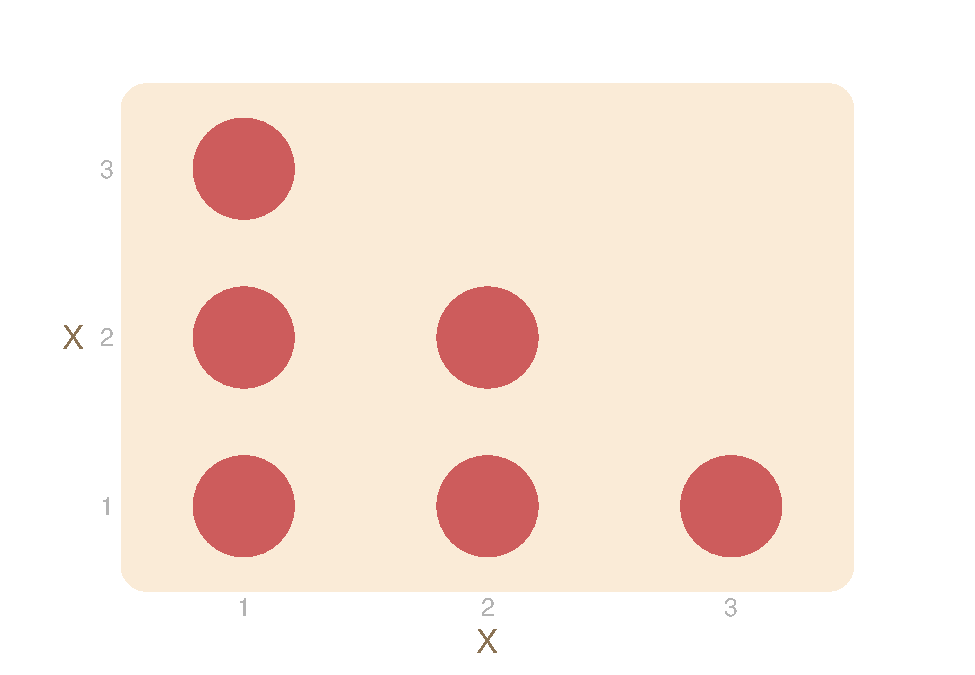
\includegraphics{_main_files/figure-latex/relations-subset-1} 

}

\caption{Relations as a subset of the Cartesian product on two sets. From the diagram, we see that 1 is less than or equal to every element of y, 2 is less than or equal to 2 and 3, and 3 is less than or equal to 3 only. Note the symmetry between rows and columns - this is due to the fact that we have the same set ($X$) on both dimensions. }\label{fig:relations-subset}
\end{figure}

Under some relation \(R\), if two elements \(x, y \in X\) relate, i.e.~if \((x, y) \in R\), we can write this using the infix notation using some infix symbol such as \(\star\): then, if \(x\) and \(y\) relate, we write \(x \star_R y\) or \(x \star y\) (\(R\) implicit). For example, for common relations such as \(=\), \(\leq\), we write \(x = y\) or \(x \leq y\). \(R\) is also sometimes used, e.g.~\(x R y\). If the elements do not relate, i.e.~\((x, y) \not \in R\), we typically do not write this out explicitly.

Relations can have properties. For example, many types of relations are \emph{reflexive}, meaning that \(x \star x\) for all \(x \in X\) (every element relates to itself). Of note, specifying three specific properties allow us to define equivalence relations:

\begin{definition}[Equivalence relation]

A relation \(\sim\) on \(X\) is called an equivalence relation if it is:

\begin{enumerate}
\def\labelenumi{\arabic{enumi}.}
\tightlist
\item
  \emph{Reflexive}: \(x \sim x\) for all \(x \in X\)
\item
  \emph{Symmetric}: \(x \sim y\) if and only if \(y \sim x\) for all \(x, y \in X\)
\item
  \emph{Transitive}: if \(x \sim y\) and \(y \sim z\), then \(x \sim z\)
\end{enumerate}

\end{definition}

Equivalence relations encode the notion that two things are \emph{same-ish}. We can further use them to assign objects in \(X\) to \emph{equivalence classes}, which group equivalent objects together. That is, for some element \(a \in X\), its corresponding equivalence class is:

\[[a] = \{ x \in X : x \sim a \}\]
We can do a lot of things with relations. The next few sections will discuss three important examples: functions, partitions, and preorders.

\subsection{Functions}\label{functions}

A function is a special kind of relation that encodes a mapping between two sets. More specifically, let \(S\) be the set of sources (also called the \emph{domain}) and \(T\) be the set of possible targets (also called the \emph{codomain}). Then, we can think of a function as a relation \(F \subseteq S \times T\) of valid source-target pairs \((s, t)\), such that for every \(s \in S\) in there exists a unique \(t \in T\) with \((s, t) \in F\) (see Figure \ref{fig:function-subset}). In other words, every source relates to exactly one target, see Figure \ref{fig:function-subset}:

\begin{figure}

{\centering 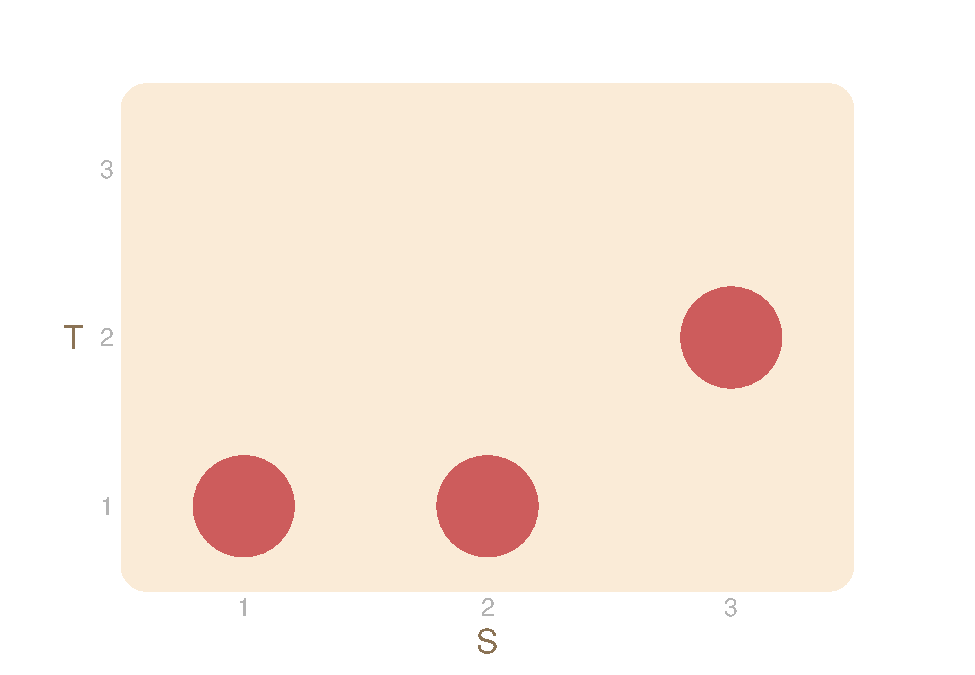
\includegraphics{_main_files/figure-latex/function-subset-1} 

}

\caption{Function as a subset of the Cartesian product on domain ($S$) and codomain ($T$). The subset $F \subseteq S \times T$ is shown in red. In words, the function is $F: \{ 1, 2, 3 \} \to \{ 1, 2, 3 \}$, such that $F(1) = 1$, $F(2) = 1$, and $F(3) = 2$, e.g. $f(x) = \lfloor x / 2 \rceil$ (divide by two and round). Note that, for any function, there must be exactly one red dot in each column (each source maps to one and only one target), however, there may be zero or many red dots in any row (some target may not be reachable, or they may be reachable from multiple sources).}\label{fig:function-subset}
\end{figure}

We can classify functions based on how their domains and codomains map onto each other (see Figure \ref{fig:function-types}). If every target in the function's codomain has a path leading to it from some source, such that no target remains unreachable, then we call it a \emph{surjective} or \emph{onto} function. More formally:

\begin{definition}[Surjectivity]
A function \(f\) is surjective if, for all \(t \in T\), there exists a \(s \in S\) such that \(f(s) = t\).
\end{definition}

Alternatively, if each source in the function's domain leads to a unique target, then we call such a function \emph{injective} or \emph{one-to-one}. That is:

\begin{definition}[Injectivity]
A function is injective if for all \(s_1, s_2 \in S\), if \(f(s_1) = t\) and \(f(s_2) = t\), then \(s_1 = s_2\).
\end{definition}

Finally, if a function is both surjective and injective, meaning that every target can be reached from, and only from, a unique source, then we call such a function \emph{bijective} or a \emph{bijection}.

\begin{definition}[Bijectivity]
A function is a bijection and only if it is both surjective and injective, and if and only if it is invertible.
\end{definition}

\begin{figure}

{\centering 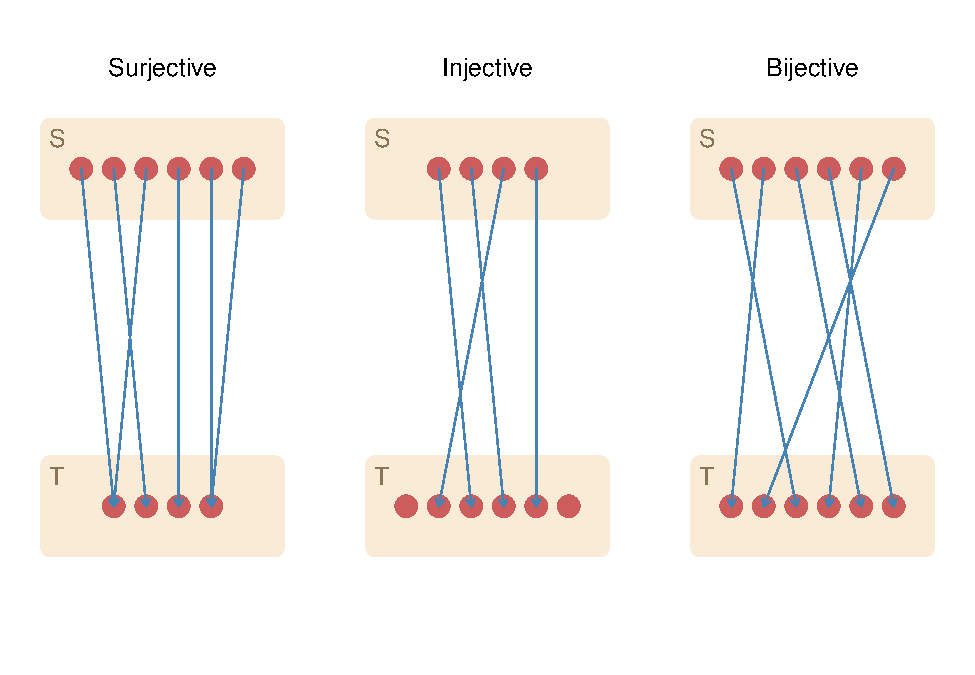
\includegraphics{_main_files/figure-latex/function-types-1} 

}

\caption{Types of functions. Left: in a *surjective* function, every target can be reached from some source. Middle: in an *injective* function, every target can only be reached from a unique source. Right: in a *bijection*, every target can be reached from, and only from, a unique source.}\label{fig:function-types}
\end{figure}

Bijections are special since they encode the idea of \emph{reversibility} or \emph{lossless transformation}. Any bijective function \(f\) has an associated inverse function \(f^{-1}\) such that \(f^{-1}(f(x)) = x\) and \(f(f^{-1}(a)) = a\) for all \(x\) and \(a\) in the function's domain and codomain, respectively, and we can keep switching back and forth from domain to codomain and back without losing any information. We'll generalize this idea later when we discuss \emph{isomorphisms}.

As an example, suppose I have a group of friends \(f \in F\) that each went to one city \(c \in C\) in Europe during the holiday. I can construct a function \(f: F \to C\) that sends each friend to his or her holiday destination. If every city in \(C\) was visited by at least one friend, then the function is surjective. If each friend went to a different destination, then the function is injective. If both are true - that is, if every city on our list was visited by exactly one friend - then the function is bijective. In that case, we could just as well use the names of cities \(c \in C\) when we speak of friends \(f \in F\) - instead of ``Sam'', we could say ``the person who went to Rome'', and it would be clear who are we talking about.

An important property of functions is that they can be composed. Specifically, if the domain of one function matches the codomain of another, the functions can be composed by piping the output of one into another to form a new function:

\begin{definition}[Function composition]

If we have two functions \(f: X \to Y\) and \(g: Y \to Z\), we can form a new function \(h: X \to Z\) such that:

\[h(x) = g(f(x))\]
We can omit the explicit reference to the variable \(x\) and write the composition in several different ways:

\begin{enumerate}
\def\labelenumi{\arabic{enumi}.}
\tightlist
\item
  \(h = g \circ f\) (read: ``apply \(g\) after \(f\)'')
\item
  \(h = gf\) (same as above)
\item
  \(h = f ⨾ g\) (read ``apply \(f\) then \(g\)'')
\end{enumerate}

\end{definition}

I will use the bracket notation (\(h(x) = g(f(x))\)) when explicitly referring to the variable, and the postfix/fat semicolon notation (\(h = f ⨾ g\)) otherwise.

There are other things we can do with functions. For example, given a subset of sources, we can ask about the \emph{image} - the set of targets we can reach from those sources:

\begin{definition}[Image]
For some subset \(S_i \subseteq S\), its image under \(f\) is defined as \(f_!(S_i) = \{ f(s) \in T \lvert s \in S_i \}\).
\end{definition}

Likewise, given a subset of targets, we can ask about the \emph{pre-image} - the set of sources that could have produced those targets. That is:

\begin{definition}[Pre-image]
For some subset \(T_i \subseteq T\), its pre-image under \(f\) is defined as \(f^*(T_i) = \{ s \in S \lvert f(s) \in T_i \}\).
\end{definition}

An important fact to note is that, although the pre-image \(f^*\) is also sometimes called ``inverse image'', it is \emph{not} the inverse of the image \(f_!\) for most functions (unless they are bijections). That is, by applying the pre-image after image or vice versa, we cannot expect to come up with the same set as we started with. Specifically, if we have a non-injective function and apply the pre-image after the image, we may come up with \emph{more} sources that we started with, \(S_i \subseteq f^*(f_!(S_i))\) (equality if injective), and similarly, if we have a non-surjective function and apply the image after the pre-image, we might end up with \emph{fewer} targets than we started with, \(f_!(f^*(T_i)) \subseteq T_i\) (again, equality if surjective).

As an example, suppose again I have the function \(f\) which maps each friend to a holiday destination. The image of that function, \(f_!\), maps a set of friends to the set of all cities that at least one of them went to, and similarly, the pre-image, \(f^*\), maps a set of cities to the set of friends that went to them.\\
Now, suppose that Sam and Dominic went to Rome, and I ask:

\begin{quote}
\emph{``who went to {[}the city that Sam went to{]}?''}
\end{quote}

I will get both Sam and Dominic back, since:

\[f^*(f_!(\{ Sam \})) = f^*(\{ Rome \}) = \{ Sam, Dominic \}\]

That is, I will get back Sam and Dominic \emph{even though I had initially only asked about Sam}. Similarly, if no friends had visited Paris and I ask:

\begin{quote}
\emph{``what are the cities that {[}people who went to Paris or Rome{]} went to?''}
\end{quote}

then I will get Rome only, since

\[f_!(f^*(\{Paris, Rome \})) = f_!(\{ Sam, Dominic \}) = \{ Rome \}\]

This weird relationship between the the image and the pre-image is due to the fact that the image is actually something called \emph{left adjoint} (\citeproc{ref-baez2023}{Baez 2023}; \citeproc{ref-fong2019}{Fong and Spivak 2019}). Adjoints can be thought of as the ``best approximate answer to a problem that has no solution'' (no inverse, \citeproc{ref-baez2023}{Baez 2023}), and they come in pairs - a left and a right adjoint - with the left adjoint being more permissive or ``liberal'' and the right adjoint being more strict or ``conservative'' (\citeproc{ref-baez2023}{Baez 2023}).

Proper treatment of adjoint is beyond the scope of this thesis, however.

\subsection{Partitions}\label{partitions}

One useful thing we can construct with functions (or equivalently, relations) are partitions. Partitions encode the idea of splitting elements of some some into distinct groups.

\begin{definition}[Function definition of a partition]
Given some set \(X\), a set of part labels \(P\), and a surjective function \(f: X \to P\), we can partition \(A\) by assigning every element \(x \in X\) a part label \(p \in P\), by simply applying the function: \(f(x) = p\).
\end{definition}

Above we used a function to define a partition, however, we can achieve the same with a relations, specifically equivalence classes. By taking any part label \(p \in P\), we can recover the corresponding subset of \(X\) by pulling out its pre-image: \(f^*(\{p\}) = X_p \subseteq X\). We can then define a partition without reference to \(f\):

\begin{definition}[Equivalence class definition of a partition]
A partition of \(A\) consists of a set of part labels \(P\), such that, for all \(p \in P\), there is a non-empty subset \(A_p \subseteq A\) which forms an equivalence class on \(A\) and:

\[X = \bigcup_{p \in P} X_p \qquad \text{and} \qquad \text{if } p \neq q, \text{ then } X_p \cap X_q = \varnothing\]
I.e. the parts \(X_p\) jointly cover the entirety of \(X\) and parts cannot share any elements.
\end{definition}

We can rank partitions by their coarseness. That is, for any set \(X\), the coarsest partition is one with only one part label \(P = \{ 1 \}\), such that each element of \(X\) gets assigned \(1\) as label. Conversely, the finest partition is one where each element gets assigned its own unique part label, such that \(\lvert X \lvert = \lvert P \lvert\).

Given two partitions, we can form a finer (or at least as fine) partition by taking their intersection, i.e.~by taking the set of all unique pairs of labels that co-occur for any \(x \in X\) as the new part labels. For example, suppose \(X = \{ 1, 2, 3 \}\) and partition 1 assigns part labels:

\[p_1(x) = \begin{cases} 
a & \text{if } x = 1 \text{ or } x = 2 \\
b & \text{if } x = 3
\end{cases}\]

and partition 2 assigns part labels the following way:

\[
p_2(a) = \begin{cases}
s & \text{if } x = 1 \\
t & \text{if } x = 2 \text{ or } x = 3
\end{cases}
\]

Then the intersection partition will have the following part labels \(P_3 = \{ (a, s), (a, t), (b, t) \}\) such that:

\[
p_3(a) = \begin{cases}
(a, s) & \text{if } x = 1 \\
(b, s) & \text{if } x = 2 \\ 
(b, t) & \text{if } x = 3
\end{cases}
\]

\subsection{Preorders}\label{preorders}

\begin{definition}[Preorder]

A preorder is a set \(X\) equipped with a binary relation \(\leq\) that conforms to two simple properties:

\begin{enumerate}
\def\labelenumi{\arabic{enumi}.}
\tightlist
\item
  \emph{Reflexivity}: \(x \leq x\) for all \(x \in X\)
\item
  \emph{Transitivity}: if \(x \leq y\) and \(y \leq z\), then \(x \leq z\), for all \(x, y, z \in X\)
\end{enumerate}

\end{definition}

Simply speaking, this means that between any two elements in \(X\), there either is a relation and the elements relate (one element is somehow ``less than or equal'' to the other), or the two elements do not relate.

An example of a preorder is the family tree, with the underlying set being the set of family members: \(X = \{  \textbf{daughter}, \textbf{son}, \textbf{mother}, \textbf{father}, \textbf{grandmother}, ... \}\) and the binary relation being ancestry or familial relation. Thus, for example, \(\textbf{daughter} \leq \textbf{father}\), since the daughter is related to the father, and \(\textbf{father} \leq \textbf{father}\), since a person is related to themselves. However, there is no relation (\(\leq\)) between \(\textbf{father}\) and \(\textbf{mother}\) since they are not related. Finally, since \(\textbf{daughter} \leq \textbf{father}\) and \(\textbf{father} \leq \textbf{grandmother}\), then, by reflexivity, \(\textbf{daughter} \leq \textbf{grandmother}\).

We can further restrict preorders by imposing additional properties, such as:

\begin{enumerate}
\def\labelenumi{\arabic{enumi}.}
\setcounter{enumi}{2}
\tightlist
\item
  If \(x \leq y\) and \(y \leq x\), then \(x = y\) (anti-symmetry)
\item
  Either \(x \leq y\) or \(y \leq x\) (comparability)
\end{enumerate}

If a preorder conforms to 3., we speak of a partially ordered set or \emph{poset}. If it conforms to both 3. and 4., then it is a \emph{total order}.

\subsection{Monoids}\label{monoids}

A monoid is a tuple \((M, e, \otimes)\) consisting of:

\begin{enumerate}
\def\labelenumi{\alph{enumi}.}
\tightlist
\item
  A set of objects \(M\)
\item
  A neutral element \(e\) called the \emph{monoidal unit}
\item
  A binary function \(\otimes: M \times M \to M\) called the \emph{monoidal product}
\end{enumerate}

Such that:

\begin{enumerate}
\def\labelenumi{\arabic{enumi}.}
\tightlist
\item
  \(m \otimes e = e \otimes m = m\) for all \(m \in M\) (unitality)
\item
  \(m_1 \otimes (m_2 \otimes m_3) = (m_1 \otimes m_2) \otimes m_3 = m_1 \otimes m_2 \otimes m_3\) for all \(m_1, m_2, m_3 \in M\) (associativity)
\end{enumerate}

In simple terms, monoids encapsulate the idea that \emph{the whole is exactly the ``sum'' of its parts} (where ``sum'' can be replaced by the monoidal product). Specifically, we have some elements and a way to combine them, and when we combine the same elements, no matter where we put the brackets we always get the same result (i.e.~something like ``the order does not matter'', although that is not precisely right, more on that later). Finally, we have some neutral element that when combined with an element yields back the same element.

For example, take summation on natural numbers, \((\mathbb{N}, 0, +)\):

\[1 + 0 = 0 + 1 = 1 \qquad \text{(unitality)}\]
\[1 + (2 + 3) = (1 + 2) + 3 = 1 + 2 + 3 \qquad \text{(associativity)}\]

Likewise, products of real numbers \((\mathbb{R}, 1, \times)\) are also a monoid, and so is multiplication of \(n \times n\) square matrices \((\mathbf{M}_{n \in \mathbb{Z}}, \mathbf{I}, \cdot)\), where \(\mathbf{I}\) is the identity matrix and \(\cdot\) stands for an infix operator that is usually omitted. As a counterexample, exponentiation does not meet the definition of a monoid, since it is not associative: \(x^{(y^z)} \neq (x^y)^z\).

There are more exotic forms of monoids as well. For example, the operation of appending a value to a vector and taking the Euclidean norm can also be recast as a monoid:

\[||(||(x, y)||_2, z)||_2 = \sqrt{\bigg(\sqrt{(x^2 + y^2)}\bigg)^2 + z^2} = \sqrt{(x^2 + y^2) + z^2} = ||(x, y, z)||_2\]

We may want to impose further restrictions on monoids, for example:

\begin{enumerate}
\def\labelenumi{\arabic{enumi}.}
\setcounter{enumi}{2}
\tightlist
\item
  \(m_1 \otimes m_2 = m_2 \otimes m_1\) for all \(m_1, m_2 \in M\) (commutativity)
\end{enumerate}

Both commutativity and associativity can both be viewed as a kind of ``order does not matter'' rule, however, they are fundamentally different. Let's imagine our set of objects consists of three wires of different colours \(\{ \textbf{red}, \textbf{green}, \textbf{blue} \}\) and the monoidal product consists of connecting wires. Let's also imagine that the \(\textbf{red}\) wire is connected to a power source and the \(\textbf{blue}\) wire is connected to a lightbulb, and the blue wire amplifies the current from the power source such that it is enough to power the light bulb. To turn on the lightbulb, we need to connect \(\textbf{red} \to \textbf{green}\) and \(\textbf{green} \to \textbf{blue}\). The time order in which we connect the three wires does not matter: we can connect \(\textbf{green} \to \textbf{blue}\) first and \(\textbf{red} \to \textbf{green}\) second or vice versa, either way we get the same result (lightbulb turns on). However, the spatial order in which we connect the wires \emph{does} matter: if we connect \(\textbf{red} \to \textbf{blue}\), then the current will not be enough to power the lightbulb. Hence, the operation is associative (temporal order does not matter) but not commutative (spatial order does matter).

If \(M\) is a preorder, another restriction we may want to impose is that the monoidal product is strictly increasing:

\begin{enumerate}
\def\labelenumi{\arabic{enumi}.}
\setcounter{enumi}{3}
\tightlist
\item
  \(m_1 \leq m_1 \otimes m_2\) and \(m_2 \leq m_1 \otimes m_2\) for all \(m_1, m_2 \in M\) (monotonicity)
\end{enumerate}

This means that when we combine two things, we get back something that's at least as big as the bigger of the two things. Summation of natural numbers \((\mathbb{N}, 0, +)\) again works, but for example summation of integers \((\mathbb{Z}, 0, +)\) or multiplication of reals \((\mathbb{R}, 1, \times)\) does not.

\section{Components of a Data Visualization System}\label{components-of-a-data-visualization-system}

\subsection{Scales}\label{scales}

Every data visualization system needs some way of translating abstract data values into concrete graphical attributes such as position, size, or colour. Given the ubiquitous need for scales, one might expect them to be a ``solved issue'', within the relevant literature. However, this is far from the truth. Specifically, the issues of scales and measurement present are still being grappled with the areas of mathematics and philosophy of science to this day (for a gentle yet thorough introduction, see \citeproc{ref-tal2015}{Tal 2015}).

Scales are another area of data visualization in which there has been considerable debate, with many terms being overloaded and relating to concepts from different fields. This is due to the fact that the issue of how to compare, rank, and translate values has a long and complicated history. In particular, the issue of measurement has been hotly debated in the field of psychometrics and mathematical psychology, leading to the development of the \emph{theory of measurement} (which has some overlap with, but is not the same as, \emph{measurement theory} in mathematics).

One paper that has been key to the debate around scales and measurement has been the seminal work of Stevens (\citeproc{ref-stevens1946}{1946}). In this paper, Stevens defined a \emph{scale} as a method of assigning numbers to values, allowing for various kinds of comparisons. Further, by considering transformations which preserve the comparisons, Stevens identified 4 types of scales: \emph{nominal}, \emph{ordinal}, \emph{interval}, and \emph{ratio} (see also \citeproc{ref-michell1986}{Michell 1986}; \citeproc{ref-velleman1993}{Velleman and Wilkinson 1993}).

\begin{table}

\caption{\label{tab:scales}Types of scales identified by Stevens (1946)}
\centering
\begin{tabular}[t]{l|l|l|l}
\hline
Scale & Structure & Comparison & Valid transformations\\
\hline
Nominal & Equivalence relation & Are \$x\$ and \$y\$ the same? & \$x' = f(x)\$ where \$f\$ is a bijection\\
\hline
Ordinal & Total order & Is \$x\$ is greater than \$y\$? & \$x' = f(x)\$ where \$f\$ is a monotonically increasing bijection\\
\hline
Interval & Lebesque measure & Is the distance from \$x\$ to \$y\$ the same as from \$a\$ to \$b\$? & \$x' = ax + b\$\\
\hline
Ratio &  & How many times is \$x\$ greater than \$y\$? & \$x' = ax\$\\
\hline
\end{tabular}
\end{table}

Table \ref{tab:scales} shows a loose reproduction of Table 1 from Stevens (\citeproc{ref-stevens1946}{1946}). Note that the family of valid transformations gets smaller in each row, meaning that the scales carry more information (\citeproc{ref-velleman1993}{Velleman and Wilkinson 1993}). Let's discuss the scales individually.

\paragraph{Nominal scales}\label{nominal-scales}

\emph{Nominal} scales correspond to equivalence relations. An equivalence relation is a binary relation \(\sim\) on some set \(X\) which, for all \(x, y, z \in X\), has the following properties:

\begin{itemize}
\tightlist
\item
  \emph{Reflexivity}: \(x \sim x\)
\item
  \emph{Symmetry}: \(x \sim y \text{ if and only if } y \sim x\)
\item
  \emph{Transitivity}: \(x \sim y \text{ and } y \sim z \text{ then } x \sim z\)
\end{itemize}

Intuitively, we can think of the numbers on a nominal scale as ``labels'', and the only question which we can ask a nominal scale is whether two labels are the same or different. A such, examples of variables with nominal scale include variables of which we typically think of as categorical, such as color, species, or political party. It does not make sense to say ``blue is \emph{more} than green'' or ``cat is \emph{more} than dog'' without specifying some other axis along which we compare. It does make sense, however, to say ``Daisy and Molly are the same species of animal (cat)'' or ``these two glasses are of different colors''.

The only transformations which are permissible for nominal scales are permutations (\citeproc{ref-stevens1946}{Stevens 1946}). For example, if we use the numbers \(\{ 1, 2, 3 \}\) to represent the species \(S = \{ \text{cat}, \text{dog}, \text{hamster} \}\), respectively, we can assign the numbers in any order we want and the properties of the scale are preserved.

It is arguable whether any nominal quantities exist in and of themselves or whether they only ever exists as abstract social constructions over underlying continuous reality. Color is a discretization of the visible light spectrum (frequency of electromagnetic radiation), and the pre-Darwinian concept of a species is likewise an abstraction over continuously varying distribution of genes (although there have been some attempts to ground the definition of a discrete species in the theory of genetics, e.g.~as a population of individuals which can produce viable offsprings, see \citeproc{ref-mayr1999}{Mayr 1999}). Further, even many subjective concepts which are typically described as discrete such as emotions may be abstractions over underlying continuous phenomena (\citeproc{ref-barrett2013}{Barrett 2013}).

However, even if nominal quantities are entirely socially constructed, this does not mean they are arbitrary or useless. SEARLE

\paragraph{Ordinal scales}\label{ordinal-scales}

\emph{Ordinal} scales correspond to total orders. A total order is a relation \(\leq\) on \(X\) which, for all \(x, y, z \in X\), has the following properties:

\begin{enumerate}
\def\labelenumi{\arabic{enumi})}
\tightlist
\item
  \emph{Reflexivity}: \(x \leq x\)
\item
  \emph{Antisymmetry}: \(\text{if } x \leq y \leq x \text{ then } x = y\)
\item
  \emph{Transitivity}: \(x \leq y \text{ and } y \leq z \text{ then } x \leq z\)
\item
  \emph{Totality} or \emph{comparability} or \emph{strong connectedness}: \(\text{for all } x, y, \text{ either } x \leq y \text{ or } y \leq x\)
\end{enumerate}

Examples of total orders include the usual ordering \(\leq\) on natural numbers \(\mathbb{N}\): \(1 \leq 2 \leq 3 \leq \ldots\) or the alphabetical order on letters: \(A \leq B \leq C \ldots \leq Z\).

As total orders, ordinal scales allow us to rank quantities. A good example of an ordinal variable is placement in a race or competition. If Emma and Charlotte ran a marathon, and Emma placed 2nd and Charlotte 3rd, we can say that Charlotte ran finished the race earlier than Emma. However, we do not know whether she crossed the finish line 15 minutes or 2 hours earlier, or whether or not her average pace was less than half of that of Emma.

Some authors have related ordinal scales to \emph{weak orders} (see \citeproc{ref-michell1986}{Michell 1986}). Weak orders (also known as \emph{total preorders}, see \citeproc{ref-nlab2024d}{nLab 2024a}) generalize total orders by allowing for ties (properties 2. and 4. above do not need hold). While this could seem desirable, I opted to relate ordinal scales to total orders here instead, since there is currently some ambiguity in the literature in the way the term \emph{weak order} is being used (see e.g. \citeproc{ref-nlab2024a}{nLab 2024b}, \citeproc{ref-nlab2024b}{2024c}; \citeproc{ref-stackexchange2024}{Abrams 2024}), and, for practical data analysis, the distinction is fairly inconsequential. For instance, in the marathon example above, if Emma and Charlotte both placed second, after Lucy and before Lily, we could frame the outcome of the race as the following weak order on the set \(M\) of marathoners: \(\text{Lucy} \leq \text{Emma, Charlotte} \leq \text{Lily} \leq ...\). However, the underlying set of ranks \(R \subset \mathbb{N}\) still retains a total ordering: \(1 \leq 2 \leq 3 \leq \ldots\) and we can specify a surjective monotonically increasing function \(r: M \to R\) which maps each marathoner to her rank. Clearly, we can map any weak order to a total order by applying a functor which enforces anti-symmetry in this way (\citeproc{ref-fong2019}{Fong and Spivak 2019}; \citeproc{ref-nlab2024d}{nLab 2024a}).

The only transformations which are permissible for ordinal scales are those which preserve order, that is, monotonic increasing transformations (\citeproc{ref-stevens1946}{Stevens 1946}; \citeproc{ref-michell1986}{Michell 1986}). For example, transforming our set of ranks \(R\) by taking the log or square root of each rank leaves the order relations between them unchanged.

\paragraph{Interval scales}\label{interval-scales}

\emph{Interval} scales.

Interval scales allow us to identify a distance between two points. However, they do not have a natural ``zero point'' or intercept. As such we cannot use them to determine the ratio between two quantities. Examples of interval scales include the calendar date and geographical position. It does not make sense to say that the year 1000 CE is ``twice'' that of 500 CE, since the birth of Jesus Christ is (one's personal religious beliefs aside) an arbitrary zero point: we could set the point 0 CE to any other event, such as the founding of Athens or the release of Taylor Swift's first album, and the ratios would be altered. Likewise, it does not make sense to say that 90° longitude is ``three times'' that of 30° longitude: the location of the prime meridian is also the product of arbitrary historical cirumstances.

\subparagraph{Ratio scales}\label{ratio-scales}

Unlike interval scales, ratio scale have a well-defined natural zero point. For example,

\paragraph{Criticism of On the Theory of Scales of Measurement}\label{criticism-of-on-the-theory-of-scales-of-measurement}

In the original paper, Stevens had also made the claim that the type of scale determined which statistical tests and summaries were ``permissible'' for the data. For example, according to Stevens, while mean is an appropriate summary of an interval scale (since expectation is linear), it would not be a permissible summary of ordinal data. This claim was later disputed by researchers

\chapter{Design}\label{design}

\subsection{User profile}\label{user-profile}

The profile of average user can also differ significantly, across systems and research areas. For example, some areas of interactive data visualization and HCI make no assumptions about the user's level of experience or motivation, whereas others assume a highly motivated ``expert'' user with a sufficient level of domain knowledge (\citeproc{ref-dimara2019}{Dimara and Perin 2019}).

While designing my system, I have attempted to

\section{Implementation}\label{implementation}

\begin{quote}
The example code chunks in this section are written in both R and TypeScript. The reason for this is that, while I would prefer to use R for everything due to its tight integration with RMarkdown, some of the concepts are much easier to explain in a language with static typing features like TypeScript (particularly, type annotations and interfaces). However, since the examples relate to plotting and some can be improved by showing graphical output/plots, I also wanted to use (base) R for plotting. So, where graphical output is important, the code chunks are written in R, and, where the code itself is the main focus, they are written in TypeScript. I hope this bilingualism is not too confusing and have tried to use only the basic features of each language to make the examples clear.
\end{quote}

\subsection{Programming paradigms}\label{programming-paradigms}

It is often the case that the same programming task can be solved in many, often vastly different, ways. Programs solving the same problem can differ in how they decompose the problem, how they represent and manipulate data, how they handle state, how explicit or implicit they are about handling low-level system details versus relying on abstractions, how they structure and organize their constituent components, and so on. Dealing with these concerns, and coming up with a formal set of principles for addressing them is the job of programming paradigms (\citeproc{ref-chambers2014}{Chambers 2014}; \citeproc{ref-jordan2015}{Jordan et al. 2015}; \citeproc{ref-van2009}{Van Roy et al. 2009}).

Most programming languages are geared towards one specific style of programming, typically supporting only one or two programming paradigms to a reasonable capacity (\citeproc{ref-van2009}{Van Roy et al. 2009}). Fortunately, this is not the case for either JavaScript/TypeScript or R, since both are multiparadigm programming languages (\citeproc{ref-chambers2014}{Chambers 2014}; \citeproc{ref-mdn2024c}{MDN 2024f}). Both support object-oriented programming, via prototype inheritance in the case of JavaScript (\citeproc{ref-mdn2024d}{MDN 2024b}) and the S3, S4, and R6 systems in the case of R (\citeproc{ref-wickham2019}{Wickham 2019}), and treat functions as first class citizens, allowing for functional programming style (\citeproc{ref-chambers2014}{Chambers 2014}; \citeproc{ref-mdn2024e}{MDN 2024d}). Further, as C based languages, both also support classical imperative/procedural programming style, and also provide some utilities for reflective metaprogramming.

The flexibility of JavaScript and R allowed me to experiment with different programming paradigms while developing \texttt{plotscaper}. I had rewritten the JavaScript side of the package multiple times from scratch, testing out several different programming paradigms and styles in the process. Below, I provide a very broad overview of the paradigms I have tried, as well as an account of my experience of using each paradigm and some thoughts on its suitability towards designing interactive data visualization systems.

\subsubsection{Imperative programming}\label{imperative-programming}

Imperative programming style is one of the oldest and most classical styles of programming. It conceptualizes the program as a discrete sequence of steps that manipulate some mutable state (\citeproc{ref-frame2014}{Frame and Coffey 2014}). In this way, it closely resembles the way CPU executes instructions.

\subsubsection{Data oriented programming}\label{data-oriented-programming}

Data oriented programming (DOP) and data oriented design (DOD) are two newer programming paradigms that have been slowly gaining prominence in the recent years. While the terms are sometimes used interchangeably, there are some subtle differences: DOP focuses more on high-level principles such as structuring and organizing code, whereas DOD, originating in the world of video-game development, tends to be more concerned with low-level optimization details such as memory layout and CPU access patterns (\citeproc{ref-sharvit2022}{Sharvit 2022}; c.f. \citeproc{ref-acton2014}{Acton 2014}; \citeproc{ref-fabian2018}{Fabian 2018}). However, there is a remarkable overlap between the conclusions and high-level concepts of the two programming paradigms. For this reason, I will discuss both here simultaneously and refer to both as ``DOP'' unless explicitly mentioned otherwise.

The core idea of DOP is a data-first perspective. Under this view, programs should be viewed as transformations of data, nothing less, nothing more. As a result, every program is composed of two sets of components: stateful data and stateless functions that transform this data (\citeproc{ref-fabian2018}{Fabian 2018}). Data should be represented by generic data structures, formed by combining maps/structs, arrays, and primitives (for example \hyperref[JSON]{JSON}; \citeproc{ref-sharvit2022}{Sharvit 2022}), and it may even be desirable that it adheres to the relational model (\citeproc{ref-codd1970}{Codd 1970}; \citeproc{ref-moseley2006}{Moseley and Marks 2006}; \citeproc{ref-fabian2018}{Fabian 2018}; note that the data does not actually have to \emph{live} inside a relational database, just have the shape of a normalized table, with columns represented by generic arrays). Data and code should be kept separate, with code living in separate modules, composed of stateless functions (\citeproc{ref-fabian2018}{Fabian 2018}; \citeproc{ref-sharvit2022}{Sharvit 2022}). Further, since data is just itself - data - there is no obligation for it to model the real world or any kind of abstract entity and we are free to represent it in any way we want (\citeproc{ref-acton2014}{Acton 2014}; \citeproc{ref-fabian2018}{Fabian 2018}; an extreme example of this are Entity Component Systems in videogames, \citeproc{ref-harkonen2019}{Härkönen 2019}). Finally, abstraction should be introduced only gradually, and most of the work should be done by generic data manipulation functions (\citeproc{ref-fabian2018}{Fabian 2018}; \citeproc{ref-sharvit2022}{Sharvit 2022}).

It may seem that many of the DOP principles directly contradict many popular OOP principles, specifically encapsulation, inheritance, polymorphism, and domain driven design. However, many of these principles can either be reconciled with DOP, or DOP in fact provides better alternatives. Below, I go over these principles and provide code examples that further illustrate how DOP works.

\paragraph{Encapsulation}\label{encapsulation}

When it comes to encapsulation in DOP, we have to differentiate between encapsulating data and encapsulating code. Encapsulating code is easy in DOP - we can simply not export certain functions from the code modules. We are then free to modify the signature of these functions without affecting the public interface (\citeproc{ref-fabian2018}{Fabian 2018}). Encapsulating data may require a bit more work. Depending on the language, generic data structures may not have property access modifiers (although there does seem to be a trend in recent languages to support property access modifiers more generically, see e.g. \citeproc{ref-rust2024}{Rust Foundation 2024}; \citeproc{ref-zig2024}{Zig Software Foundation 2024}). For instance, in JavaScript, private properties can only be declared as part of a class declaration (\citeproc{ref-mdn2024e}{MDN 2024d}). However, in most languages, it is still possible to use other language features and metaprogramming to achieve data encapsulation - for example, in JavaScript, we can use the Proxy class to emulate private property access (\hyperref[dop-encapsulation]{see Appendix}).

Thus, encapsulation of data is certainly possible in DOP. However, a question still remains whether it is a good idea. Encapsulation is generally seen as a net positive in OOP, however, in the DOP view, data encapsulation presents trade-offs. While it may provide an additional layer of security, it also makes systems more complex and harder to debug (\citeproc{ref-fabian2018}{Fabian 2018}; \citeproc{ref-sharvit2022}{Sharvit 2022}). , And, even with fully encapsulated data, users may still come to rely on hidden features of the system (\citeproc{ref-fabian2018}{Fabian 2018}). Ultimately, it is necessary to weigh the pros and cons of encapsulating data within the context of the specific use-case.

In JavaScript, there is also a third option which I actually found to be a good fit while writing \texttt{plotscape}, and that is a weak form of encapsulation by using symbol keys (\citeproc{ref-mdn2024f}{MDN 2024c}). Symbols are builtin primitive that are guaranteed to be unique. By not exporting the symbol value, we can make a property weakly encapsulated in the sense that the user will not be able to access it without using reflection. For example:

\begin{Shaded}
\begin{Highlighting}[]
\CommentTok{// Meta.ts}
\KeywordTok{const}\NormalTok{ METADATA }\OperatorTok{=} \BuiltInTok{Symbol}\NormalTok{(}\StringTok{"metadata"}\NormalTok{)}\OperatorTok{;}
\KeywordTok{type}\NormalTok{ METADATA }\OperatorTok{=} \KeywordTok{typeof}\NormalTok{ METADATA}\OperatorTok{;}

\ImportTok{export} \KeywordTok{interface}\NormalTok{ Meta}\OperatorTok{\textless{}}\NormalTok{T }\KeywordTok{extends} \BuiltInTok{Record}\OperatorTok{\textless{}}\DataTypeTok{string}\OperatorTok{,} \DataTypeTok{any}\OperatorTok{\textgreater{}} \OperatorTok{=} \DataTypeTok{any}\OperatorTok{\textgreater{}}\NormalTok{ \{}
\NormalTok{  [METADATA]}\OperatorTok{:}\NormalTok{ T}\OperatorTok{;}
\NormalTok{\}}

\ImportTok{export} \ImportTok{namespace} \DataTypeTok{Meta}\NormalTok{ \{}
  \ImportTok{export} \KeywordTok{function} \KeywordTok{of}\OperatorTok{\textless{}}\NormalTok{T }\KeywordTok{extends} \BuiltInTok{Object}\OperatorTok{\textgreater{}}\NormalTok{(object}\OperatorTok{:}\NormalTok{ T) \{}
    \ControlFlowTok{return}\NormalTok{ \{ }\OperatorTok{...}\KeywordTok{object}\OperatorTok{,}\NormalTok{ [METADATA]}\OperatorTok{:}\NormalTok{ \{\} \}}\OperatorTok{;}
\NormalTok{  \}}

  \ImportTok{export} \KeywordTok{function} \KeywordTok{get}\OperatorTok{\textless{}}\NormalTok{T }\KeywordTok{extends}\NormalTok{ Meta}\OperatorTok{\textgreater{}}\NormalTok{(object}\OperatorTok{:}\NormalTok{ T}\OperatorTok{,}\NormalTok{ key}\OperatorTok{:} \KeywordTok{keyof}\NormalTok{ T[METADATA]) \{}
    \ControlFlowTok{return} \KeywordTok{object}\NormalTok{[METADATA][key]}\OperatorTok{;}
\NormalTok{  \}}

  \ImportTok{export} \KeywordTok{function} \KeywordTok{set}\OperatorTok{\textless{}}\NormalTok{T }\KeywordTok{extends}\NormalTok{ Meta}\OperatorTok{,}\NormalTok{ K }\KeywordTok{extends} \KeywordTok{keyof}\NormalTok{ T[METADATA]}\OperatorTok{\textgreater{}}\NormalTok{(}
\NormalTok{    object}\OperatorTok{:}\NormalTok{ T}\OperatorTok{,}
\NormalTok{    key}\OperatorTok{:}\NormalTok{ K}\OperatorTok{,}
\NormalTok{    value}\OperatorTok{:}\NormalTok{ T[METADATA][K]}
\NormalTok{  ) \{}
    \KeywordTok{object}\NormalTok{[METADATA][key] }\OperatorTok{=}\NormalTok{ value}\OperatorTok{;}
\NormalTok{  \}}
\NormalTok{\}}
\end{Highlighting}
\end{Shaded}

Now we can import the module and use it to add secret metadata to arbitrary data objects:

\begin{Shaded}
\begin{Highlighting}[]
\ImportTok{import}\NormalTok{ \{ Meta \} }\ImportTok{from} \StringTok{"./Meta.ts"}

\KeywordTok{interface}\NormalTok{ User }\KeywordTok{extends}\NormalTok{ Meta}\OperatorTok{\textless{}}\NormalTok{\{ id}\OperatorTok{:} \DataTypeTok{number}\NormalTok{ \}}\OperatorTok{\textgreater{}}\NormalTok{ \{}
\NormalTok{  name}\OperatorTok{:} \DataTypeTok{string}\OperatorTok{;}
\NormalTok{\}}

\KeywordTok{const}\NormalTok{ user}\OperatorTok{:}\NormalTok{ User }\OperatorTok{=}\NormalTok{ Meta}\OperatorTok{.}\FunctionTok{of}\NormalTok{(\{ name}\OperatorTok{:} \StringTok{"Adam"}\NormalTok{ \})}\OperatorTok{;}
\NormalTok{Meta}\OperatorTok{.}\FunctionTok{set}\NormalTok{(user}\OperatorTok{,} \VerbatimStringTok{\textasciigrave{}id\textasciigrave{}}\OperatorTok{,} \DecValTok{1337}\NormalTok{)}\OperatorTok{;}
\BuiltInTok{console}\OperatorTok{.}\FunctionTok{log}\NormalTok{(Meta}\OperatorTok{.}\FunctionTok{get}\NormalTok{(user}\OperatorTok{,} \VerbatimStringTok{\textasciigrave{}id\textasciigrave{}}\NormalTok{))}\OperatorTok{;}

\KeywordTok{interface}\NormalTok{ Variable }\KeywordTok{extends} \BuiltInTok{Array}\OperatorTok{\textless{}}\DataTypeTok{number}\OperatorTok{\textgreater{},}\NormalTok{ Meta}\OperatorTok{\textless{}}\NormalTok{\{ min}\OperatorTok{:} \DataTypeTok{number}\OperatorTok{;}\NormalTok{ max}\OperatorTok{:} \DataTypeTok{number}\NormalTok{ \}}\OperatorTok{\textgreater{}}\NormalTok{ \{\}}

\KeywordTok{const}\NormalTok{ values}\OperatorTok{:}\NormalTok{ Variable }\OperatorTok{=}\NormalTok{ Meta}\OperatorTok{.}\FunctionTok{of}\NormalTok{([}\DecValTok{1}\OperatorTok{,} \DecValTok{2}\OperatorTok{,} \DecValTok{3}\NormalTok{])}\OperatorTok{;}
\NormalTok{Meta}\OperatorTok{.}\FunctionTok{set}\NormalTok{(values}\OperatorTok{,} \VerbatimStringTok{\textasciigrave{}min\textasciigrave{}}\OperatorTok{,} \DecValTok{0}\NormalTok{)}\OperatorTok{;}
\BuiltInTok{console}\OperatorTok{.}\FunctionTok{log}\NormalTok{(Meta}\OperatorTok{.}\FunctionTok{get}\NormalTok{(values}\OperatorTok{,} \VerbatimStringTok{\textasciigrave{}min\textasciigrave{}}\NormalTok{))}\OperatorTok{;}
\end{Highlighting}
\end{Shaded}

The user can access and set the metadata values using the \texttt{Meta.get} and \texttt{Meta.set} functions, however, they cannot directly access the metadata property since the value \texttt{METADATA} symbol is not exported. There is a way to access this symbol via the \texttt{Reflect.ownKeys} and \texttt{Object.getOwnPropertySymbols} functions, and so this is not a strong form of encapsulation (\citeproc{ref-mdn2024f}{MDN 2024c}). However, arguably, if the user goes as far as to use these functions, and, assuming we are not storing any sensitive data (which is generally not the case in interactive data visualization), it may be reasonable to allow them to access these ``private'' values and suffer the consequences.

\paragraph{Inheritance}\label{inheritance}

In OOP, the primary mechanism for code reuse is inheritance.

In DOP, since data is generic and separate from behavior, we can call functions from any module as long as the data we provide it as arguments adheres to the module's interface. This makes code reuse trivial. For example, here's a simplified version of the \texttt{Reactive} interface (Observer pattern) from \texttt{plotscape}:

\begin{Shaded}
\begin{Highlighting}[]

\KeywordTok{const}\NormalTok{ LISTENERS }\OperatorTok{=} \BuiltInTok{Symbol}\NormalTok{(}\VerbatimStringTok{\textasciigrave{}listeners\textasciigrave{}}\NormalTok{)}\OperatorTok{;} \CommentTok{// A unique symbol, to avoid namespace clashes}
\KeywordTok{type}\NormalTok{ Dict }\OperatorTok{=} \BuiltInTok{Record}\OperatorTok{\textless{}}\DataTypeTok{string}\OperatorTok{,} \DataTypeTok{any}\OperatorTok{\textgreater{};} \CommentTok{// Generic dictionary type}
\KeywordTok{type}\NormalTok{ Callback }\OperatorTok{=}\NormalTok{ (data}\OperatorTok{:}\NormalTok{ Dict) }\KeywordTok{=\textgreater{}} \DataTypeTok{void}\OperatorTok{;} \CommentTok{// Generic callback function type}

\KeywordTok{interface}\NormalTok{ Reactive \{}
\NormalTok{  [LISTENERS]}\OperatorTok{:} \BuiltInTok{Record}\OperatorTok{\textless{}}\DataTypeTok{string}\OperatorTok{,}\NormalTok{ Callback[]}\OperatorTok{\textgreater{};}
\NormalTok{\}}

\ImportTok{namespace} \DataTypeTok{Reactive}\NormalTok{ \{}
  \ImportTok{export} \KeywordTok{function} \KeywordTok{of}\OperatorTok{\textless{}}\NormalTok{T }\KeywordTok{extends} \BuiltInTok{Object}\OperatorTok{\textgreater{}}\NormalTok{(object}\OperatorTok{:}\NormalTok{ T)}\OperatorTok{:}\NormalTok{ T }\OperatorTok{\&}\NormalTok{ Reactive \{}
    \ControlFlowTok{return}\NormalTok{ \{ }\OperatorTok{...}\KeywordTok{object}\OperatorTok{,}\NormalTok{ [LISTENERS]}\OperatorTok{:}\NormalTok{ \{\} \}}\OperatorTok{;}
\NormalTok{  \}}

  \ImportTok{export} \KeywordTok{function} \FunctionTok{listen}\NormalTok{(object}\OperatorTok{:}\NormalTok{ Reactive}\OperatorTok{,}\NormalTok{ event}\OperatorTok{:} \DataTypeTok{string}\OperatorTok{,}\NormalTok{ cb}\OperatorTok{:}\NormalTok{ Callback) \{}
    \ControlFlowTok{if}\NormalTok{ (}\OperatorTok{!}\KeywordTok{object}\NormalTok{[LISTENERS][}\BuiltInTok{event}\NormalTok{]) }\KeywordTok{object}\NormalTok{[LISTENERS][}\BuiltInTok{event}\NormalTok{] }\OperatorTok{=}\NormalTok{ []}\OperatorTok{;}
    \KeywordTok{object}\NormalTok{[LISTENERS][}\BuiltInTok{event}\NormalTok{]}\OperatorTok{.}\FunctionTok{push}\NormalTok{(cb)}\OperatorTok{;}
\NormalTok{  \}}

  \ImportTok{export} \KeywordTok{function} \FunctionTok{dispatch}\NormalTok{(object}\OperatorTok{:}\NormalTok{ Reactive}\OperatorTok{,}\NormalTok{ event}\OperatorTok{:} \DataTypeTok{string}\OperatorTok{,}\NormalTok{ data}\OperatorTok{:}\NormalTok{ Dict) \{}
    \ControlFlowTok{for}\NormalTok{ (}\KeywordTok{const}\NormalTok{ cb }\KeywordTok{of} \KeywordTok{object}\NormalTok{[LISTENERS][}\BuiltInTok{event}\NormalTok{] }\OperatorTok{??}\NormalTok{ []) }\FunctionTok{cb}\NormalTok{(data)}\OperatorTok{;}
\NormalTok{  \}}
\NormalTok{\}}

\KeywordTok{interface}\NormalTok{ Dog }\KeywordTok{extends}\NormalTok{ Reactive \{}
\NormalTok{  name}\OperatorTok{:} \DataTypeTok{string}
\NormalTok{\}}

\ImportTok{namespace} \DataTypeTok{Dog}\NormalTok{ \{}
  \ImportTok{export} \KeywordTok{function} \KeywordTok{of}\NormalTok{(name}\OperatorTok{:} \DataTypeTok{string}\NormalTok{) \{}
    \ControlFlowTok{return}\NormalTok{ Reactive}\OperatorTok{.}\FunctionTok{of}\NormalTok{(\{ name \})}
\NormalTok{  \}}
\NormalTok{\}}

\KeywordTok{const}\NormalTok{ dog }\OperatorTok{=}\NormalTok{ Dog}\OperatorTok{.}\FunctionTok{of}\NormalTok{(}\VerbatimStringTok{\textasciigrave{}Terry\textasciigrave{}}\NormalTok{)}
\NormalTok{Reactive}\OperatorTok{.}\FunctionTok{listen}\NormalTok{(dog}\OperatorTok{,} \VerbatimStringTok{\textasciigrave{}car goes by\textasciigrave{}}\OperatorTok{,}\NormalTok{ () }\KeywordTok{=\textgreater{}} \BuiltInTok{console}\OperatorTok{.}\FunctionTok{log}\NormalTok{(}\VerbatimStringTok{\textasciigrave{}Woof!\textasciigrave{}}\NormalTok{))}
\NormalTok{Reactive}\OperatorTok{.}\FunctionTok{dispatch}\NormalTok{(dog}\OperatorTok{,} \VerbatimStringTok{\textasciigrave{}car goes by\textasciigrave{}}\NormalTok{)}
\end{Highlighting}
\end{Shaded}

\begin{verbatim}
## Woof!
\end{verbatim}

\section{System components}\label{system-components}

\subsection{Factors}\label{factors}

Factors provide a way to partition the data into multiple disjoint parts.

\subsubsection{Product factors}\label{product-factors}

We can combine a factor with \(j\) levels and another factor with \(k\) levels into a product factor with up to \(j \cdot k\) levels.

I independently discovered a formula similar to (\citeproc{ref-wickham2013}{Wickham 2013}):

\[i_{\text{product}} = i_1 + i_2 \cdot \max(j, k)\]

\subsection{Reducers}\label{reducers}

(\citeproc{ref-gray1997}{Gray et al. 1997}) came up with OLAP data cube

\subsection{Scales}\label{scales-1}

A fundamental task when visualizing data is translating values from the coordinates of the data to something that can be actually displayed on the screen. In most data visualization system, this is the job of scales. While there exists is a fair amount of literature on the theoretical properties of scales {[}SEE INTRODUCTION{]}, there is much less written about the actual details of implementing scales in concrete data visualization systems. As such, the following section is based largely on how scales have been implemented in other data visualization codebases, such as the \texttt{ggplot2} R package (\citeproc{ref-wickham2016}{Wickham 2016}) or \texttt{d3-scale} module of D3 (\citeproc{ref-d3-scale2024}{Observable 2024}), as well on personal insights while implementing the package.

\subsubsection{Overview}\label{overview}

From a high-level perspective, we can think of a scale as just a function \(s: D \to V\), which translates data values \(d \in D\) to some visual attribute (co)domain \(V\), which could be, for example, the x- or y-position, length, area, radius, or color.

The simplest and most typical case is where both \(S\) and \(D\) are subsets of the real numbers:

\[s: [d_{min}, d_{max}] \to [v_{min}, v_{max}] \qquad d_{min}, d_{max}, v_{min}, v_{max} \in \mathbb{R}\]

For example, suppose our data takes values in the range from 1 to 10 and we want to plot it along the x-axis within a plotting region which is 800 pixels wide. Then, our scale is simply:

\[s: [1, 10] \to [0, 800]\]

Now, there can be many potential functions that fit this signature. One particularly nice and simple candidate is the following function:

\[s(d) = v_{max} + \frac{d - d_{min}}{d_{max} - d_{min}} \cdot (v_{max} - v_{min})\]

or, with concrete values substituted for the variables:

\[s(d) = 0 + \frac{d - 1}{10 - 1} \cdot (800 - 0) \\ \implies s(d) = [(d - 1) / 9] \cdot 800\]

This function is a simple linear map, which acts on the data in the following way:

\begin{itemize}
\tightlist
\item
  \(s(1) = (1 - 1) / 9 \cdot 800 = 0\)
\item
  \(s(10) = (10 - 1) / 9 \cdot 800 = 800\)
\item
  \(s(d) \in (0, 800)\) for any \(d \in (1, 10)\)
\end{itemize}

That is, the function maps the data value 1 to pixel 0 (left border of the plotting region), value 10 to to pixel 800 (right border of the plotting region), and any value in between 1 and 10 to the interval 0 to 800, proportional to where in the data range it is located.

We can easily implement the function by simply translating the formula to code:

\begin{Shaded}
\begin{Highlighting}[]
\KeywordTok{function} \FunctionTok{scale}\NormalTok{(}
\NormalTok{  d}\OperatorTok{:} \DataTypeTok{number}\OperatorTok{,}
\NormalTok{  dmin}\OperatorTok{:} \DataTypeTok{number}\OperatorTok{,}
\NormalTok{  dmax}\OperatorTok{:} \DataTypeTok{number}\OperatorTok{,}
\NormalTok{  vmin}\OperatorTok{:} \DataTypeTok{number}\OperatorTok{,}
\NormalTok{  vmax}\OperatorTok{:} \DataTypeTok{number}\OperatorTok{,}
\NormalTok{)}\OperatorTok{:} \DataTypeTok{number}\NormalTok{ \{}
  \ControlFlowTok{return}\NormalTok{ vmin }\OperatorTok{+}\NormalTok{ ((d }\OperatorTok{{-}}\NormalTok{ dmin) }\OperatorTok{/}\NormalTok{ (dmax }\OperatorTok{{-}}\NormalTok{ dmin)) }\OperatorTok{*}\NormalTok{ (vmax }\OperatorTok{{-}}\NormalTok{ vmin)}\OperatorTok{;}
\NormalTok{\}}

\CommentTok{// And indeed, this works as expected}
\BuiltInTok{console}\OperatorTok{.}\FunctionTok{log}\NormalTok{(}\FunctionTok{scale}\NormalTok{(}\FloatTok{5.5}\OperatorTok{,} \DecValTok{1}\OperatorTok{,} \DecValTok{10}\OperatorTok{,} \DecValTok{0}\OperatorTok{,} \DecValTok{800}\NormalTok{))}
\end{Highlighting}
\end{Shaded}

\begin{verbatim}
## 400
\end{verbatim}

\subsubsection{Limits of modeling scales as simple functions}\label{limits-of-modeling-scales-as-simple-functions}

Simple scale functions like the one shown above can work fine for basic data visualization systems. However, once we want to add more features, this design can become prohibitive. Consider, for example, what we might have to do if we want to:

\begin{itemize}
\tightlist
\item
  Expand the scale limits
\item
  Apply non-linear transformations
\item
  Pan, zoom, reversem, or otherwise modify the scale interactively
\item
  Scale discrete data
\end{itemize}

Let's take the first point as a motivating example. Consider what happens to data points at the limits of the data range with our ``simple'' scale function:

\begin{Shaded}
\begin{Highlighting}[]
\NormalTok{x }\OtherTok{\textless{}{-}} \DecValTok{1}\SpecialCharTok{:}\DecValTok{10}
\NormalTok{y }\OtherTok{\textless{}{-}} \FunctionTok{rnorm}\NormalTok{(}\DecValTok{10}\NormalTok{, }\DecValTok{0}\NormalTok{, }\DecValTok{5}\NormalTok{)}
\NormalTok{col }\OtherTok{\textless{}{-}} \FunctionTok{ifelse}\NormalTok{(}\DecValTok{1}\SpecialCharTok{:}\DecValTok{10} \SpecialCharTok{\%in\%} \FunctionTok{c}\NormalTok{(}\DecValTok{1}\NormalTok{, }\DecValTok{10}\NormalTok{), }\StringTok{"indianred"}\NormalTok{, }\StringTok{"grey80"}\NormalTok{)}

\FunctionTok{plot}\NormalTok{(x, y, }\AttributeTok{col =}\NormalTok{ col, }\AttributeTok{cex =} \DecValTok{3}\NormalTok{, }\AttributeTok{xaxs =} \StringTok{"i"}\NormalTok{)}
\end{Highlighting}
\end{Shaded}

\begin{center}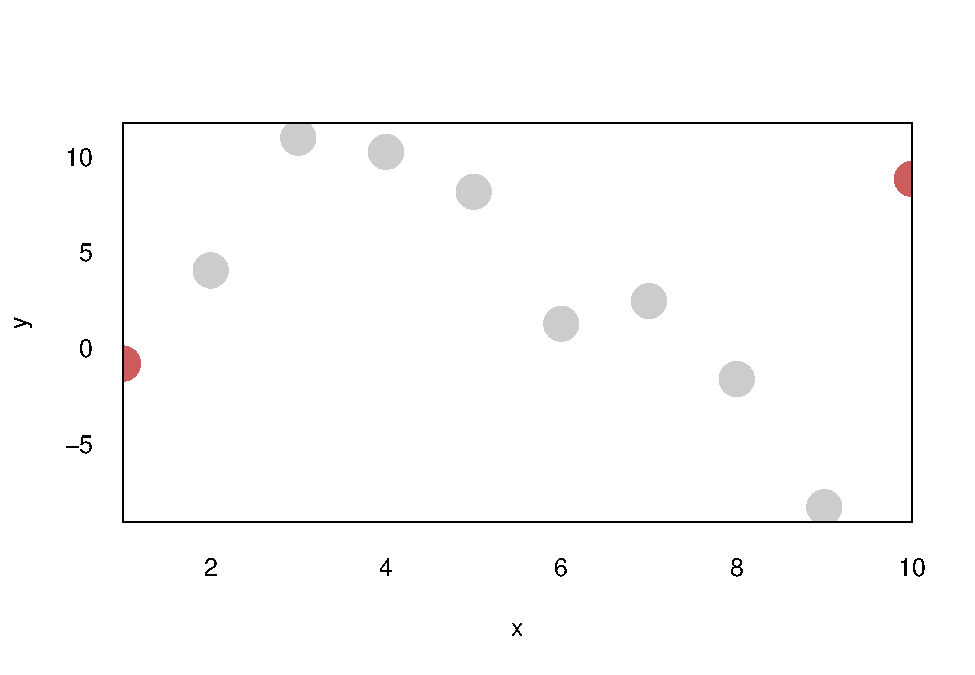
\includegraphics[width=800px]{_main_files/figure-latex/unnamed-chunk-7-1} \end{center}

The plot above shows values scaled using the simple linear mapping described above along the x-axis, i.e.~\(s: [1, 10] \to [0, 800]\). Notice that, since the position of the points representing the values 1 and 10 get mapped to pixel values 0 and 800 (the left and right border of the plot), only half of each point is visible.

To address this, most data visualization systems automatically expand the range of the domain by some pre-specified percentage:

\begin{Shaded}
\begin{Highlighting}[]
\FunctionTok{plot}\NormalTok{(x, y, }\AttributeTok{col =}\NormalTok{ col, }\AttributeTok{cex =} \DecValTok{3}\NormalTok{)}
\end{Highlighting}
\end{Shaded}

\begin{center}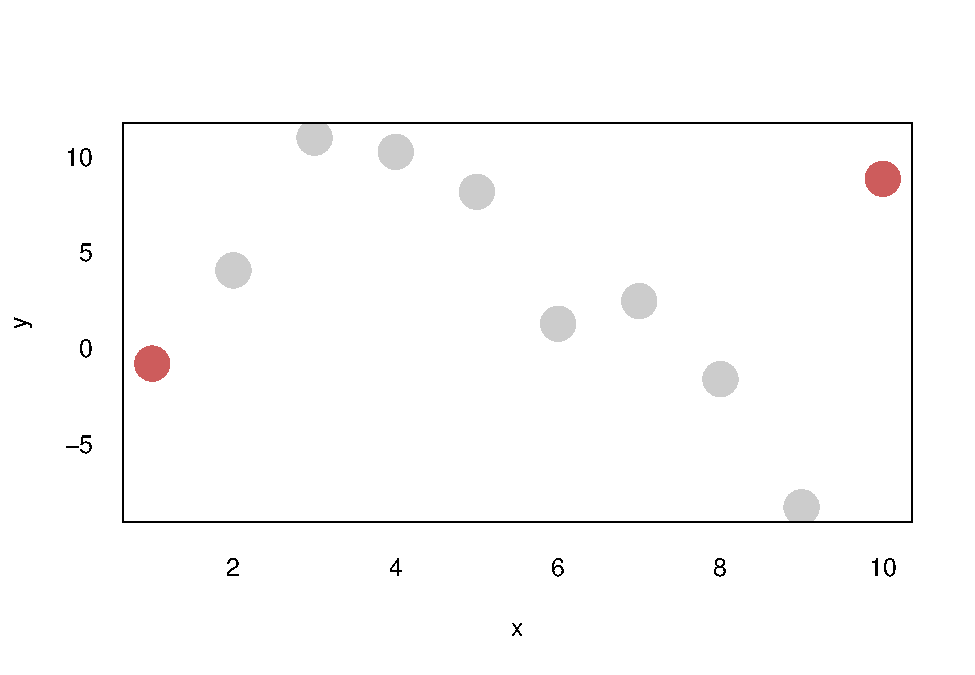
\includegraphics[width=800px]{_main_files/figure-latex/unnamed-chunk-8-1} \end{center}

(in R, this is approximately 4\% at each end of the axis, see \texttt{xaxs} in \texttt{?graphicss::par})

Turning back to the simple \texttt{scale} function, we could achieve the same effect by adding an extra argument:

\begin{Shaded}
\begin{Highlighting}[]
\KeywordTok{function} \FunctionTok{scale}\NormalTok{(}
\NormalTok{  d}\OperatorTok{:} \DataTypeTok{number}\OperatorTok{,}
\NormalTok{  dmin}\OperatorTok{:} \DataTypeTok{number}\OperatorTok{,}
\NormalTok{  dmax}\OperatorTok{:} \DataTypeTok{number}\OperatorTok{,}
\NormalTok{  vmin}\OperatorTok{:} \DataTypeTok{number}\OperatorTok{,}
\NormalTok{  vmax}\OperatorTok{:} \DataTypeTok{number}\OperatorTok{,}
\NormalTok{  exp}\OperatorTok{:} \DataTypeTok{number}\OperatorTok{,}
\NormalTok{)}\OperatorTok{:} \DataTypeTok{number}\NormalTok{ \{}
  \ControlFlowTok{return}\NormalTok{ (}
\NormalTok{    vmin }\OperatorTok{+}\NormalTok{ (exp }\OperatorTok{/} \DecValTok{2} \OperatorTok{+}\NormalTok{ ((d }\OperatorTok{{-}}\NormalTok{ dmin) }\OperatorTok{/}\NormalTok{ (dmax }\OperatorTok{{-}}\NormalTok{ dmin)) }\OperatorTok{*}\NormalTok{ (}\DecValTok{1} \OperatorTok{{-}}\NormalTok{ exp)) }\OperatorTok{*}\NormalTok{ (vmax }\OperatorTok{{-}}\NormalTok{ vmin)}
\NormalTok{  )}\OperatorTok{;}
\NormalTok{\}}

\BuiltInTok{console}\OperatorTok{.}\FunctionTok{log}\NormalTok{(}\FunctionTok{scale}\NormalTok{(}\DecValTok{1}\OperatorTok{,} \DecValTok{1}\OperatorTok{,} \DecValTok{10}\OperatorTok{,} \DecValTok{0}\OperatorTok{,} \DecValTok{800}\OperatorTok{,} \FloatTok{0.1}\NormalTok{))}\OperatorTok{;}
\BuiltInTok{console}\OperatorTok{.}\FunctionTok{log}\NormalTok{(}\FunctionTok{scale}\NormalTok{(}\FloatTok{5.5}\OperatorTok{,} \DecValTok{1}\OperatorTok{,} \DecValTok{10}\OperatorTok{,} \DecValTok{0}\OperatorTok{,} \DecValTok{800}\OperatorTok{,} \FloatTok{0.1}\NormalTok{))}\OperatorTok{;}
\BuiltInTok{console}\OperatorTok{.}\FunctionTok{log}\NormalTok{(}\FunctionTok{scale}\NormalTok{(}\DecValTok{10}\OperatorTok{,} \DecValTok{1}\OperatorTok{,} \DecValTok{10}\OperatorTok{,} \DecValTok{0}\OperatorTok{,} \DecValTok{800}\OperatorTok{,} \FloatTok{0.1}\NormalTok{))}\OperatorTok{;}
\end{Highlighting}
\end{Shaded}

\begin{verbatim}
## 40
## 400
## 760
\end{verbatim}

The \texttt{exp} argument effectively allows allows us expand the data range by some fixed percentage, e.g.~10\% (5\% upper and lower limit, respectively). This means that the data values of 1 and 10 are no longer translated to 0 and 800 pixels but instead somewhere closer to the center of the plotting area (40 and 760 pixels, respectively).

However, as can be plainly seen, with more arguments, the function quickly becomes unwieldy and hard to reason about. Further, we also may want to persist or modify some of the values during runtime (such as when panning or zooming). Therefore, a more structured approach is needed.

\subsubsection{Solution: Two-component scale system}\label{solution-two-component-scale-system}

The linear mapping formula can guide us in decomposing the scaling function into smaller, more manageable parts. Looking at the formula closely, we can see that it can be expressed as the composition of two simpler functions:

\[s(x) = \color{steelblue}{j +} \color{indianred}{\frac{x - a}{b -a}} \color{steelblue}{\cdot (k - j)}\]

That is, the scale function consists of:

\begin{itemize}
\tightlist
\item
  A \emph{normalize} function \(\color{indianred}{n: D \to [0, 1], \qquad n(d) = (d - a) / (b - a)}\)
\item
  An \emph{unnormalize} function \(\color{steelblue}{u: [0, 1] \to V, \qquad u(p) = j + p \cdot (k - j)}\)
\end{itemize}

Put simply, the normalize function \(n\) translates data values \(d \in D\) to a percentage \(p \in [0, 1]\), and the unnormalize function \(u\) converts the percentage to the space of the visual attribute \(V\). The scale function is then simply the composition of these two functions:

\[s(d) = \color{steelblue}{u(} \color{indianred}{n(\color{black}{d})} \color{steelblue}{)}\]

In code, we can write this as follows:

\begin{Shaded}
\begin{Highlighting}[]
\KeywordTok{function} \FunctionTok{normalize}\NormalTok{(x}\OperatorTok{:} \DataTypeTok{number}\OperatorTok{,}\NormalTok{ a}\OperatorTok{:} \DataTypeTok{number}\OperatorTok{,}\NormalTok{ b}\OperatorTok{:} \DataTypeTok{number}\NormalTok{) \{}
  \ControlFlowTok{return}\NormalTok{ (x }\OperatorTok{{-}}\NormalTok{ a) }\OperatorTok{/}\NormalTok{ (b }\OperatorTok{{-}}\NormalTok{ a)}
\NormalTok{\}}

\KeywordTok{function} \FunctionTok{unnormalize}\NormalTok{(p}\OperatorTok{:} \DataTypeTok{number}\OperatorTok{,}\NormalTok{ j}\OperatorTok{:} \DataTypeTok{number}\OperatorTok{,}\NormalTok{ k}\OperatorTok{:} \DataTypeTok{number}\NormalTok{) \{}
 \ControlFlowTok{return}\NormalTok{ j }\OperatorTok{+}\NormalTok{ p }\OperatorTok{*}\NormalTok{ (k }\OperatorTok{{-}}\NormalTok{ j) }
\NormalTok{\}}

\BuiltInTok{console}\OperatorTok{.}\FunctionTok{log}\NormalTok{(}\FunctionTok{normalize}\NormalTok{(}\FloatTok{5.5}\OperatorTok{,} \DecValTok{1}\OperatorTok{,} \DecValTok{10}\NormalTok{))}
\BuiltInTok{console}\OperatorTok{.}\FunctionTok{log}\NormalTok{(}\FunctionTok{unnormalize}\NormalTok{(}\FloatTok{0.5}\OperatorTok{,} \DecValTok{0}\OperatorTok{,} \DecValTok{800}\NormalTok{))}
\end{Highlighting}
\end{Shaded}

\begin{verbatim}
## 0.5
## 400
\end{verbatim}

This two component system allows for a clean separation of concerns. Specifically, the normalize function how to map the data values to \([0, 1]\). It does not need to be aware of where these normalized data values will be mapped to. Conversely, the unnormalize function only needs to understand how to translate values from \([0, 1]\) to the space of the visual attribute (such as x-axis position).

It is worth noting that any finite subset of \(\mathbb{R}\) could serve as the intermediate domain. However, the specific interval \([0, 1]\) is convenient, both in terms of interpretation as well as for implementation, as will be discussed later.

Finally, so far I have referred to the normalize and unnormalize \emph{functions}. Framing scales as composition of functions leads to a nice correspondence between the mathematical definition and the code implementation. However, in practice, we can just as well implement the domain and codomain as \emph{objects} or \emph{classes}, as we will see in the next section. The important point is that, no matter what type the two components are, each is responsible for translating values between its domain and the interval \([0, 1]\).

\subsubsection{Past implementations of scales}\label{past-implementations-of-scales}

Implementing scales as composition of two components is fairly standard across data visualization packages. For example, the D3 library (\citeproc{ref-bostock2011}{Michael Bostock, Ogievetsky, and Heer 2011}) implements scales in a functional style, with the values representing the data domain and the visual (co)domain being provided as tuples or arrays of values, either during initialization or at some later point. For illustration, here are some examples from the oficial documentation (\citeproc{ref-d3-scale2024}{Observable 2024}):

\begin{Shaded}
\begin{Highlighting}[]
\CommentTok{// const x = d3.scaleLinear([10, 130], [0, 960]);}
\CommentTok{// x(20); // 80}
\CommentTok{// const y = d3.scaleLinear().domain([10, 130]);}
\end{Highlighting}
\end{Shaded}

Internally, specialized functions are then used to translate from the domain to the codomain, such as the \texttt{normalize()} and \texttt{scale()} functions for continuous and discrete/ordinal domains, respectively, and various \texttt{interpolate()} functions for codomains.

Similarly, \texttt{ggplot2} (\citeproc{ref-wickham2016}{Wickham 2016}) implements each subtype of the \texttt{Scale} class with \texttt{limits} and \texttt{palette} properties, each corresponding roughly to the data domain and the visual codomain (``roughly'', because the x- and y-position are treated slightly differently, due to being passed through coordinate systems). Internally, the package uses the \texttt{rescale} function from the \texttt{scales} package (\citeproc{ref-wickham2023}{Wickham, Pedersen, and Seidel 2023}) to map data to \([0, 1]\) and then the palette function is responsible for mapping these normalized values to the visual attribute. For illustration, here's the full definition of the \texttt{map} method on the \texttt{ScaleContinuous} class (I've added my own comments for clarity):

\begin{Shaded}
\begin{Highlighting}[]
\NormalTok{map }\OtherTok{=} \ControlFlowTok{function}\NormalTok{(self, x, }\AttributeTok{limits =}\NormalTok{ self}\SpecialCharTok{$}\FunctionTok{get\_limits}\NormalTok{()) \{}
  \CommentTok{\# Limits are just a tuple, rescale maps x to [0, 1]}
\NormalTok{  x }\OtherTok{\textless{}{-}}\NormalTok{ self}\SpecialCharTok{$}\FunctionTok{rescale}\NormalTok{(self}\SpecialCharTok{$}\FunctionTok{oob}\NormalTok{(x, }\AttributeTok{range =}\NormalTok{ limits), limits) }

\NormalTok{  uniq }\OtherTok{\textless{}{-}} \FunctionTok{unique0}\NormalTok{(x)}
  \CommentTok{\# Palette is a function which returns a vector of attribute values}
\NormalTok{  pal }\OtherTok{\textless{}{-}}\NormalTok{ self}\SpecialCharTok{$}\FunctionTok{palette}\NormalTok{(uniq) }
\NormalTok{  scaled }\OtherTok{\textless{}{-}}\NormalTok{ pal[}\FunctionTok{match}\NormalTok{(x, uniq)]}

  \FunctionTok{ifelse}\NormalTok{(}\SpecialCharTok{!}\FunctionTok{is.na}\NormalTok{(scaled), scaled, self}\SpecialCharTok{$}\NormalTok{na.value)}
\NormalTok{\}}
\end{Highlighting}
\end{Shaded}

\subsubsection{Proposed model of scales}\label{proposed-model-of-scales}

One disadvantage the models of scales that \texttt{D3} and \texttt{ggplot2} use is that they treat the data domain and the visual attribute codomain as fundamentally different objects. In \texttt{D3}, different functions are used to translate from \(D \to [0, 1]\) and from \([0, 1] \to V\), and, in \texttt{ggplot2}, while \texttt{limits} is a simple vector/tuple, \texttt{palette} is a function. While this approach may have some benefits, it does add additional complexity, since we have to use a different mental model when considering each component. Further, the model only works in one direction, for mapping values \(D \to V\); if we want to go the other way, i.e.~map \(V \to D\), we have to use other specialized functions.

Instead, I propose a different model of scales which implements both the domain and codomain as objects of the same type (\texttt{Expanse}). This has the advantage of making the code easier to reason about, and, most of the time, inverting the scaling function is trivial.

Here is a (somewhat) simplified version of the \texttt{Scale} interface:

\begin{Shaded}
\begin{Highlighting}[]
\KeywordTok{interface}\NormalTok{ Scale}\OperatorTok{\textless{}}\NormalTok{D}\OperatorTok{,}\NormalTok{ V}\OperatorTok{\textgreater{}}\NormalTok{ \{}
\NormalTok{  domain}\OperatorTok{:}\NormalTok{ Expanse}\OperatorTok{\textless{}}\NormalTok{D}\OperatorTok{\textgreater{}}
\NormalTok{  codomain}\OperatorTok{:}\NormalTok{ Expanse}\OperatorTok{\textless{}}\NormalTok{V}\OperatorTok{\textgreater{}}
\NormalTok{\}}
\end{Highlighting}
\end{Shaded}

Here, \texttt{D} represents the type of the data domain, and \texttt{V} represents the type of the visual attribute codomain.

With this interface, we can use of the following two functions:

\begin{Shaded}
\begin{Highlighting}[]
\KeywordTok{function} \FunctionTok{pushforward}\OperatorTok{\textless{}}\NormalTok{D}\OperatorTok{,}\NormalTok{ D}\OperatorTok{\textgreater{}}\NormalTok{(scale}\OperatorTok{:}\NormalTok{ Scale}\OperatorTok{\textless{}}\NormalTok{D}\OperatorTok{,}\NormalTok{ V}\OperatorTok{\textgreater{},}\NormalTok{ value}\OperatorTok{:}\NormalTok{ D)}\OperatorTok{:}\NormalTok{ V}
\KeywordTok{function} \FunctionTok{pullback}\OperatorTok{\textless{}}\NormalTok{D}\OperatorTok{,}\NormalTok{ V}\OperatorTok{\textgreater{}}\NormalTok{(scale}\OperatorTok{:}\NormalTok{ Scale}\OperatorTok{\textless{}}\NormalTok{D}\OperatorTok{,}\NormalTok{ V}\OperatorTok{\textgreater{},}\NormalTok{ value}\OperatorTok{:}\NormalTok{ V)}\OperatorTok{:}\NormalTok{ D}
\end{Highlighting}
\end{Shaded}

The \texttt{pushforward} function can be \emph{push values forward} through the scale, first through its domain and then its codomain, and the \texttt{pullback} function can be used to \emph{pull values back}, first through its codomain and then through its domain. The implementation of these functions is actually trivial:

\begin{Shaded}
\begin{Highlighting}[]
\KeywordTok{function} \FunctionTok{pushforward}\OperatorTok{\textless{}}\NormalTok{D}\OperatorTok{,}\NormalTok{ V}\OperatorTok{\textgreater{}}\NormalTok{(scale}\OperatorTok{:}\NormalTok{ Scale}\OperatorTok{\textless{}}\NormalTok{D}\OperatorTok{,}\NormalTok{ V}\OperatorTok{\textgreater{},}\NormalTok{ value}\OperatorTok{:}\NormalTok{ D)}\OperatorTok{:}\NormalTok{ V \{}
  \ControlFlowTok{return} \FunctionTok{unnormalize}\NormalTok{(scale}\OperatorTok{.}\AttributeTok{codomain}\OperatorTok{,} \FunctionTok{normalize}\NormalTok{(scale}\OperatorTok{.}\AttributeTok{domain}\OperatorTok{,}\NormalTok{ value))}
\NormalTok{\}}

\KeywordTok{function} \FunctionTok{pullback}\OperatorTok{\textless{}}\NormalTok{D}\OperatorTok{,}\NormalTok{ V}\OperatorTok{\textgreater{}}\NormalTok{(scale}\OperatorTok{:}\NormalTok{ Scale}\OperatorTok{\textless{}}\NormalTok{D}\OperatorTok{,}\NormalTok{ V}\OperatorTok{\textgreater{},}\NormalTok{ value}\OperatorTok{:}\NormalTok{ V)}\OperatorTok{:}\NormalTok{ D \{}
  \ControlFlowTok{return} \FunctionTok{unnormalize}\NormalTok{(scale}\OperatorTok{.}\AttributeTok{domain}\OperatorTok{,} \FunctionTok{normalize}\NormalTok{(scale}\OperatorTok{.}\AttributeTok{codomain}\OperatorTok{,}\NormalTok{ value))}
\NormalTok{\}}
\end{Highlighting}
\end{Shaded}

That is, each \texttt{Expanse} does all of the work, translating between either \(D\) or \(V\) and \([0, 1]\); a \texttt{Scale} only connects two arbitrary expanses together. As such, before talking about additional features of scales, we should discuss expanses, since these lend scale the bulk of their functionality.

\subsection{Expanses}\label{expanses}

As was hinted at in the previous section, expanses map values between their domain and the interval \([0, 1]\). To do this, they are equipped with two familiar functions:

\begin{itemize}
\tightlist
\item
  A \emph{normalize} function \(\color{indianred}{n: X \to [0, 1]}\)
\item
  An \emph{unnormalize} function \(\color{steelblue}{u: [0, 1] \to X}\)
\end{itemize}

Or, in code:

\begin{Shaded}
\begin{Highlighting}[]
\KeywordTok{function} \FunctionTok{normalize}\OperatorTok{\textless{}}\NormalTok{X}\OperatorTok{\textgreater{}}\NormalTok{(expanse}\OperatorTok{:}\NormalTok{ Expanse}\OperatorTok{\textless{}}\NormalTok{X}\OperatorTok{\textgreater{},}\NormalTok{ value}\OperatorTok{:}\NormalTok{ X)}\OperatorTok{:} \DataTypeTok{number}
\KeywordTok{function} \FunctionTok{unnnormalize}\OperatorTok{\textless{}}\NormalTok{X}\OperatorTok{\textgreater{}}\NormalTok{(expanse}\OperatorTok{:}\NormalTok{ Expanse}\OperatorTok{\textless{}}\NormalTok{X}\OperatorTok{\textgreater{},}\NormalTok{ value}\OperatorTok{:} \DataTypeTok{number}\NormalTok{)}\OperatorTok{:}\NormalTok{ X}
\end{Highlighting}
\end{Shaded}

Notice that, whereas before we had considered \emph{normalize} as mapping between \(D \to [0, 1]\) and \emph{unnormalize} as mapping between \([0, 1] \to V\), we now consider both as mapping between \([0, 1]\) and an arbitrary domain \(X\). This domain can represent the data or the visual attribute - the expanse is agnostic about this.

Also, while before we have discussed domains as subsets of \(\mathbb{R}\), we can now start thinking about them as arbitrary sets. While subsets of \(\mathbb{R}\) and sets of strings are really the only types of domains used in \texttt{plotscaper}, the model should readily extends to other sets, as long as a mapping to and from \([0, 1]\) can be provided.

How \texttt{normalize} and \texttt{unnormalize} are implemented will depend largely on the subtype of \texttt{Expanse}, as well as on the desired behavior. For example, as will be discussed later, in \texttt{plotscaper}, the normalize and unnormalize methods implemented for \texttt{ExpanseContinuous} (subtype of \texttt{Expanse\textless{}number\textgreater{}}) work largely the same way as in section {[}SECTION{]}. However, while \texttt{ExpansePoint} and \texttt{ExpanseBand} are both subtypes of \texttt{Expanse\textless{}string\textgreater{}}, they behave differently - \texttt{ExpansePoint} maps strings (factor levels) to equidistant points along \([0, 1]\), whereas \texttt{ExpanseBand} maps the strings into the middle of ``buckets'' along \([0, 1]\).

However, there is also some behavior that we may want to apply the same way across the different expanse subtypes. For example, it seems reasonable that the user should be able to zoom, pan, or reverse axes, regardless of whether a plot shows discrete or continuous data. As such, there may be some properties and functions common to the \texttt{Expanse} type. I will discuss these first.

\subsubsection{Zero and one}\label{zero-and-one}

The maps may also take in and return values outside of \(D^*\) and \([0, 1]\), if adjustments have been made. For instance, in most data visualization packages, x- and y-axis limits are by default expanded some percentage beyond the range of the observed data to avoid the maximum and minimum datapoints from overlapping with the limits. For example, in base R:

\begin{Shaded}
\begin{Highlighting}[]
\FunctionTok{set.seed}\NormalTok{(}\DecValTok{12345}\NormalTok{)}
\NormalTok{x }\OtherTok{\textless{}{-}} \FunctionTok{rnorm}\NormalTok{(}\DecValTok{5}\NormalTok{)}
\NormalTok{y }\OtherTok{\textless{}{-}} \FunctionTok{rnorm}\NormalTok{(}\DecValTok{5}\NormalTok{)}

\FunctionTok{par}\NormalTok{(}\AttributeTok{mfrow =} \FunctionTok{c}\NormalTok{(}\DecValTok{1}\NormalTok{, }\DecValTok{2}\NormalTok{))}
\FunctionTok{plot}\NormalTok{(x, y) }
\FunctionTok{plot}\NormalTok{(x, y, }\AttributeTok{xaxs =} \StringTok{\textquotesingle{}i\textquotesingle{}}\NormalTok{, }\AttributeTok{yaxs =} \StringTok{\textquotesingle{}i\textquotesingle{}}\NormalTok{) }
\end{Highlighting}
\end{Shaded}

\begin{figure}

{\centering 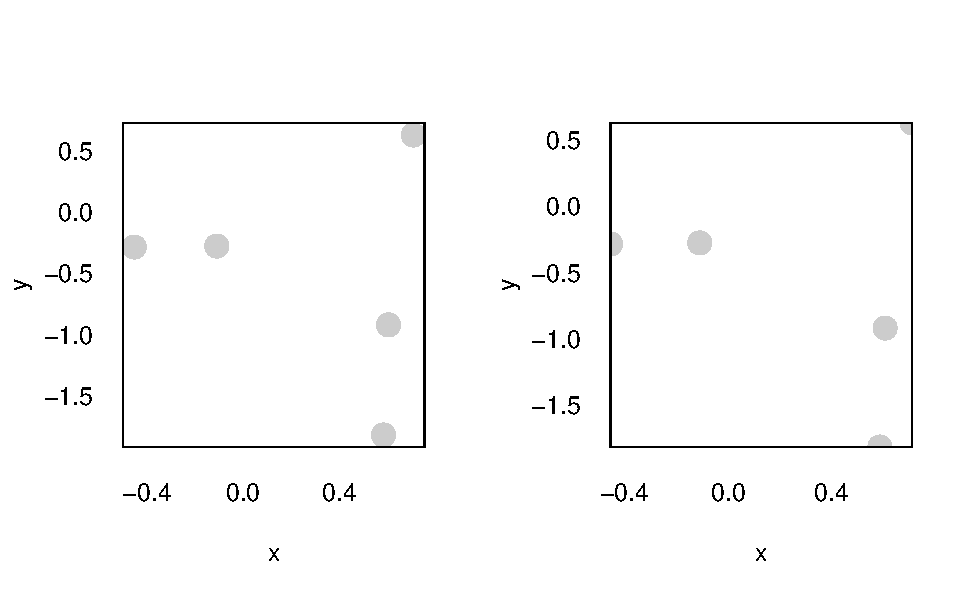
\includegraphics{_main_files/figure-latex/unnamed-chunk-17-1} 

}

\caption{Expanding axes. By default, axes in base R `plot()` function are expanded 4\% beyond the range of the data (left). Otherwise, datapoints on the limits of their respective scales end up overlapping with the plot borders (right).}\label{fig:unnamed-chunk-17}
\end{figure}

Thus, upon normalizing the minimum and maximum data values, the expanse should return values other than \(\{0, 1\}\). Likewise, to support user interactions such as zooming and panning, the expanses may accept and return values outside of \(D^*\) and \([0, 1]\).

Zooming and panning should be orthogonal to the underlying data type, such that user can interact with the plots the same way\footnote{The one exception may be panning barplots and histograms, where the y-axis upper y-axis limit may change but the lower should be fixed at 0, such that panning may shrink or stretch the bars, but not ``lift'' them up or move them down.}, no matter whether their axes are continuous, discrete, or some combination of the two. To this end, I introduce two parameters representing the normalized value (\(p\)) of the minimum and maximum data point, called \emph{zero} and \emph{one} respectively. These parameters are agnostic to the underlying data type, such that if we have the data type-specific maps \(n'\) and \(u'\), the complete normalize and unnormalize maps are:

\[n(d) = \text{zero} + n'(d) \cdot (\text{one} - \text{zero})\]
\[u(p) = u' \bigg(\frac{p - \text{zero}}{\text{one} - \text{zero}} \bigg)\]

To simplify, here's what effect setting the two parameters to specific values has:

\begin{tabular}{r|r|l}
\hline
Zero & One & Effect\\
\hline
0.05 & 0.95 & Expands the margins by \textasciitilde{}5\% (actually 5.555...\% since 0.05 / 0.9 = 0.0555...)\\
\hline
0.05 & 1.05 & Shifts the expanse 'up' by 5\% (e.g. moves x-axis 5\% right)\\
\hline
-0.50 & 1.50 & Zooms into the middle 50\% of the expanse (25 percentile goes to 0 and 75th to one)\\
\hline
\end{tabular}

\subsubsection{Expanse Interface}\label{expanse-interface}

There are also other behaviours that expanses should support. For instance, we may want to be able to reset the expanse to defaults, retrain when the underlying data changes, and return nicely formatted breaks. How these behaviours are implemented, as well as other types of behavior, may be specific to the underlying data type. Overall, expanse interface may look something like this:

\begin{verbatim}
interface Expanse<T> {
  normalize(value: T): number
  unnormalize(value: number): T
  defaultize(): this
  
  setZero(zero: number, default: boolean): this
  setOne(one: number, default: boolean): this
  freezeZero(): this
  freezeOne(): this
  
  move(amount: number): this
  expand(zero: number, one: number): this
  
  retrain(values: T[]): this
  breaks(n?: number): T[]  
}
\end{verbatim}

\subsubsection{Continuous Expanses}\label{continuous-expanses}

The continuous expanse has as its underlying set \([\min, \max] \subseteq \mathbb{R}\). To understand how it works, let's build it step by step.

We start with the basic normalizing function:

\begin{enumerate}
\def\labelenumi{\arabic{enumi}.}
\tightlist
\item
  \[n(d) = \frac{d - \min}{\max - \min}\]
\end{enumerate}

This function takes some data value \(d \in [\min, \max]\) and transforms it to \([0, 1]\). Most data visualization systems use a function like this at some step of the scaling processs - see \href{https://github.com/r-lib/scales/blob/84560bf54e02315477a05384ee67991e9e8fc52c/R/bounds.R\#L85}{\texttt{scales::rescale}} and \textbf{D3} \href{https://github.com/d3/d3-scale/blob/d6904a4bde09e16005e0ad8ca3e25b10ce54fa0d/src/continuous.js\#L122}{\texttt{normalize}}.

This may work well for typical linear scales. However, we may also want to apply some transformation \(f\), such as square root or log. Then, to ensure that the observed data values still get normalized to \([0, 1]\), we need to apply the transformation to both \(d\) and the limits:

\begin{enumerate}
\def\labelenumi{\arabic{enumi}.}
\setcounter{enumi}{1}
\tightlist
\item
  \[\frac{f(d) - f(\min)}{f(\max) - f(\min)}\]
\end{enumerate}

Finally, as was discussed in \hyperref[expanses]{EXPANSES}, we want to be able to incorporate the zero and one paramaters, leading to the final normalizing function:

\[n(d) = \text{zero} + \frac{f(d) - f(\min)}{f(\max) - f(\min)} \cdot (\text{zero} - \text{one})\]

To obtain the unnormalizing function, we can simply invert the normalizing function:

\[u(p) = f^{-1} \bigg\{ f(\min) + \frac{p - \text{zero}}{\text{one} - \text{zero}} \cdot \big[ f(\max) - f(\min) \big] \bigg\}\]

The function transforms \(x\) to a percentage value \(p \in [0, 1]\), provided \(x\) is within \([\min, \max]\). The value \((\max - \min)\) is also sometimes called the \emph{range} (not to be confused with \textbf{D3} \texttt{range}).

We can invert the normalizing function and obtain the unnormalizing function, which is, for some percentage \(p \in [0, 1]\):

\[u(p) = \min + p \cdot (\max - \min)\]
returns a value within the \([\min, \max]\) range, corresponding to the proportion of the maximum possible distance (range) from the origin (\(\min\)). For example, \(u(0.5)\), returns a value that is located halfway between the limits.

We can implement a simple continuous expanse like so:

\begin{Shaded}
\begin{Highlighting}[]

\KeywordTok{function} \FunctionTok{identity}\OperatorTok{\textless{}}\NormalTok{T}\OperatorTok{\textgreater{}}\NormalTok{(x}\OperatorTok{:}\NormalTok{ T) \{}
  \ControlFlowTok{return}\NormalTok{ x}\OperatorTok{;}
\NormalTok{\}}

\KeywordTok{function} \FunctionTok{expanseContinuous}\NormalTok{(min }\OperatorTok{=} \DecValTok{0}\OperatorTok{,}\NormalTok{ max }\OperatorTok{=} \DecValTok{1}\NormalTok{) \{}
  \KeywordTok{const}\NormalTok{ [zero}\OperatorTok{,}\NormalTok{ one] }\OperatorTok{=}\NormalTok{ [}\DecValTok{0}\OperatorTok{,} \DecValTok{1}\NormalTok{]}
  \KeywordTok{const}\NormalTok{ [trans}\OperatorTok{,}\NormalTok{ inv] }\OperatorTok{=}\NormalTok{ [identity}\OperatorTok{,}\NormalTok{ identity]}
  
  \ControlFlowTok{return}\NormalTok{ \{ min}\OperatorTok{,}\NormalTok{ max}\OperatorTok{,}\NormalTok{ zero}\OperatorTok{,}\NormalTok{ one}\OperatorTok{,}\NormalTok{ trans}\OperatorTok{,}\NormalTok{ inv}\OperatorTok{,}
    \FunctionTok{range}\NormalTok{() \{}
      \ControlFlowTok{return} \KeywordTok{this}\OperatorTok{.}\AttributeTok{max} \OperatorTok{{-}} \KeywordTok{this}\OperatorTok{.}\AttributeTok{min}\OperatorTok{;}
\NormalTok{    \}}\OperatorTok{,}
    \FunctionTok{transRange}\NormalTok{() \{}
      \KeywordTok{const}\NormalTok{ \{ min}\OperatorTok{,}\NormalTok{ max}\OperatorTok{,}\NormalTok{ trans \} }\OperatorTok{=} \KeywordTok{this}\OperatorTok{;}
      \ControlFlowTok{return} \FunctionTok{trans}\NormalTok{(max) }\OperatorTok{{-}} \FunctionTok{trans}\NormalTok{(min)}\OperatorTok{;}
\NormalTok{    \}}\OperatorTok{,}
    \FunctionTok{normalize}\NormalTok{(x}\OperatorTok{:} \DataTypeTok{number}\NormalTok{) \{}
      \KeywordTok{const}\NormalTok{ \{ min}\OperatorTok{,}\NormalTok{ zero}\OperatorTok{,}\NormalTok{ one}\OperatorTok{,}\NormalTok{ trans \} }\OperatorTok{=} \KeywordTok{this}\OperatorTok{;}
      \KeywordTok{const}\NormalTok{ normalized }\OperatorTok{=}\NormalTok{ (}\FunctionTok{trans}\NormalTok{(x) }\OperatorTok{{-}} \FunctionTok{trans}\NormalTok{(min)) }\OperatorTok{/} \KeywordTok{this}\OperatorTok{.}\FunctionTok{transRange}\NormalTok{()}\OperatorTok{;}
      \ControlFlowTok{return}\NormalTok{ zero }\OperatorTok{+}\NormalTok{ normalized }\OperatorTok{*}\NormalTok{ (one }\OperatorTok{{-}}\NormalTok{ zero)}\OperatorTok{;}
\NormalTok{    \}}\OperatorTok{,}
    \FunctionTok{unnormalize}\NormalTok{(p}\OperatorTok{:} \DataTypeTok{number}\NormalTok{) \{}
      \KeywordTok{const}\NormalTok{ \{ min}\OperatorTok{,}\NormalTok{ zero}\OperatorTok{,}\NormalTok{ one}\OperatorTok{,}\NormalTok{ trans}\OperatorTok{,}\NormalTok{ inv \} }\OperatorTok{=} \KeywordTok{this}\OperatorTok{;}
      \ControlFlowTok{return} \FunctionTok{inv}\NormalTok{(}\FunctionTok{trans}\NormalTok{(min) }\OperatorTok{+}\NormalTok{ ((p }\OperatorTok{{-}}\NormalTok{ zero) }\OperatorTok{/}\NormalTok{ (one }\OperatorTok{{-}}\NormalTok{ zero)) }\OperatorTok{*} \KeywordTok{this}\OperatorTok{.}\FunctionTok{transRange}\NormalTok{())}\OperatorTok{;}
\NormalTok{    \}}\OperatorTok{,}
\NormalTok{  \}}\OperatorTok{;}
\NormalTok{\}}

\KeywordTok{const}\NormalTok{ expanse1 }\OperatorTok{=} \FunctionTok{expanseContinuous}\NormalTok{(}\DecValTok{1}\OperatorTok{,} \DecValTok{10}\NormalTok{)}\OperatorTok{;}

\BuiltInTok{console}\OperatorTok{.}\FunctionTok{log}\NormalTok{(expanse1}\OperatorTok{.}\FunctionTok{normalize}\NormalTok{(}\DecValTok{5}\NormalTok{))}\OperatorTok{;}
\BuiltInTok{console}\OperatorTok{.}\FunctionTok{log}\NormalTok{(expanse1}\OperatorTok{.}\FunctionTok{unnormalize}\NormalTok{(}\FloatTok{0.5}\NormalTok{))}
\end{Highlighting}
\end{Shaded}

\begin{verbatim}
## 0.4444444444444444
## 5.5
\end{verbatim}

The functions \(n, u\) have several interesting properties. First off, they are inverses to each other and form an \emph{isomorphism}, i.e.~\(u = n^{-1}\) and \(n = u^{-1}\) such that \(u(n(x)) = x\) and \(n(u(p)) = p\). This also means that each function is a 1-to-1 mapping or \emph{bijection}. In plain words, this means that we cannot get the same percentage by normalizing two different values and vice versa. As a result, we can keep switching between the normalized and unnormalized representations without losing any information:

\paragraph{Linearity}\label{linearity}

Another important thing to note is that, while these types of normalizing functions are often called ``linear'' (e.g.~\texttt{scaleLinear()} in \textbf{D3}), since their graphs form a straight line, they should not be confused with ``linear functions'', since they do not satisfy the properties of linear functions, namely:

\begin{itemize}
\tightlist
\item
  Additivity: \(\text{normalize}(x + c) \neq \text{normalize}(x) + \text{normalize}(c)\)
\item
  Homogeneity of degree 1: \(\text{normalize}(c \cdot x) \neq c \cdot \text{normalize(x)}\).
\end{itemize}

To illustrate, additivity does not hold when \(\min \neq 0\) because:

\[\frac{(x + c) - \min}{(\max - \min)}\]
\[= \frac{x - \min}{\max - \min} + \frac{c}{\max - \min}\]
\[\neq \frac{x - \min}{\max - min} + \frac{c - \min}{\max - \min}\]

The same can be easily shown for the \(\text{unnormalize}\) map and for homogeneity.

Technically, this is due to a confusion between the definition of a ``linear function'' and a ``linear polynomial''. The appropriate term to use would actually be ``affine transformation.''

Either way, if the minimum is not 0, we cannot expect the following to be equal:

Or the following to be equal:

However, if we keep in mind the fact that the normalizing function calculates the proportion of distance from the origin, we can see that the function in fact behaves linearly within the context of its limits.

For example, consider the range \([1, 10]\). The value \(5\) is \(4\) units away from the lower limit, i.e.~\(5 - 1 = 4\), so we can represent it, for example, as the sum of a value that is 3 units away and another that is one unit away, \(n(5) = n(4) + n(2)\):

Likewise, again because \(5\) represents the distance of \(4\) units and \(3\) of \(2\), we can expect \(n(5) = 2 \cdot n(3)\):

\paragraph{Transformations}\label{transformations}

We can apply transformations to continuous expanses by transforming their limits. The outcome of this is that \(\min\) and \(\max\) still get mapped to \(0\) and \(1\) however, the graph of the function is no longer linear. Suppose we have non-linear function \(f\), along with an inverse \(f^{-1}\). Then:

\[n(x) = \frac{f(x) - f(\min)}{f(\max) - f(\min)}\]
\[u(p) = f^{-1} \bigg\{f(\min) + p \cdot \big[ f(\max) - f(\min) \big] \bigg\}\]
For example, here's how we could apply the transformation \(\bigg( f(x) = \sqrt{x}, \; f^{-1}(x) = x^2 \bigg)\) in code:

Transformations such as these can be useful in two ways. First, sometimes we may be able to better see trends in the data when the data has been appropriately transformed. This is the case, for example, when plotting data which varies across orders of magnitude. In this case it may be useful to apply \(\log\)-transformation. Second, transformations can also be helpful in situations where some graphical attributes are not perceived linearly. For example, when judging differently sized objects, viewers tend judge magnitude based on area rather than side or radius. As such, when drawing objects such as points or squares it can be helpful to apply square root as the inverse transformation. The idea is that, if one point has a data value that is \(c\) times bigger than another, it will have \(\sqrt{c}\) times bigger radius and \(c\) times bigger area. Note that we are talking about the inverse transformation here, i.e.~the transformation affecting the unnormalizing function.

One thing to note is that the proportionality of the square-root transformation holds only when \(\min = 0\). Otherwise:

\[\sqrt{(\min)^2 + cp \cdot [(\max)^2 - (\min)^2]}\]
\[= \sqrt{c} \cdot \sqrt{(\min)^2/c + p \cdot [(\max)^2 - (\min)^2]}\]
\[\neq \sqrt{c} \cdot \sqrt{(\min)^2 + p \cdot [(\max)^2 - (\min)^2]}\]

This is a problem in the existing packages. For example:

\section{}\label{section}

\chapter{Glossary}\label{glossary}

\subsubsection{JSON}\label{JSON}

Short for ``JavaScript Object Notation'', JSON is a flexible data format based on the JavaScript object type (\citeproc{ref-ecma2024}{Ecma International 2024}; see also e.g. \citeproc{ref-bourhis2017}{Bourhis et al. 2017}; \citeproc{ref-pezoa2016}{Pezoa et al. 2016}). On the highest level, a JSON is an dictionary (also known as object, struct, hash-table, or list in other languages) containing key-value pairs, where the keys are strings and the values can be any of the following types: string, number, boolean, null (an undefined/missing value), an array (which can contain any other valid JSON values), or another JSON object.

For example, the following snippet is a valid JSON:

\begin{verbatim}
{
  "name": "Adam",
  "age": 30,
  "friends": [{ "name": "Sam", "age": 30 }, { "name": "Franta", "age": 26}],
  "can drive": true,
  "problems": null
}
\end{verbatim}

JSON is more limited than a true JavaScript object type (as implemented in the browser and various JavaScript runtimes). JavaScript objects are very flexible and can have non-string keys (numbers or symbols) and contain a wider variety of values, most notably functions/methods (and, of course, both the keys and values can be changed during runtime). In contrast, JSON is a ``simple'' static data format designed for declaring and transporting data. Specifically, JSON is often used as the medium for sending data to and from Web APIs (\citeproc{ref-bourhis2017}{Bourhis et al. 2017}; \citeproc{ref-pezoa2016}{Pezoa et al. 2016}) as well as for configuration documents.

The main advantages of JSON are that it is a simple, flexible, and human-readable format. Also, due to its recursive nature (JSON arrays and objects can contain other JSON arrays and objects), it can be used to express a wide variety of hierarchical data which would not be efficient to express in ``flat'' data formats such as CSV. However, this flexibility also comes with some disadvantages. The recursive nature of the format makes parsing JSON files inherently more time-intensive, and, since the values in a JSON can be of any type (as long as it is a valid JSON type), it is often necessary to validate JSON data inputs (\citeproc{ref-pezoa2016}{Pezoa et al. 2016}).

\subsubsection{SVG}\label{svg}

Short for ``Scalable Vector Graphics'', SVG is a markup language for defining vector graphics (\citeproc{ref-mdn2024b}{MDN 2024e}). Based on XML, SVG graphics can be specified via a hierarchy of elements enclosed by tags, which may be given attributes.

For example, the following is a valid SVG:

\begin{verbatim}
<svg width="400" height="400">
  <circle cx="200" cy="200" r="50" fill="skyblue"></circle>
  <rect x="150" y="150" width="50" height="50" fill="firebrick"></rect>
</svg>
\end{verbatim}

And this is its output, as interpreted by a Web browser:

Compared to typical raster formats such as PNG or JPEG, in which the image is defined as an array of pixels or bytes, SVG has the advantage that its lossless: images can be arbitrarily scaled or transformed without loss of quality. SVG images can also be easily manipulated and animated by modifying the elements' attributes (for example, to move the red rectangle in the image above to the right, we could simply increment its ``x'' attribute). However, the main disadvantage of SVG is that the file size scales with the number of objects in the image. As such, SVG images with many small objects (such as points on a scatterplot) can become prohibitively large and slow to render.

\chapter{Appendix}\label{appendix}

\subsubsection{Encapsulation in DOP}\label{dop-encapsulation}

For example, here's how we can emulate private property access in JavaScript using Proxy. We create a namespace with a single constructor function that takes an object and a namespace and returns a proxy of the object which prevents access to the object fields outside of the namespace:

\begin{Shaded}
\begin{Highlighting}[]
\CommentTok{// Private.ts}
\ImportTok{export} \ImportTok{namespace} \DataTypeTok{Private}\NormalTok{ \{}
  \ImportTok{export} \KeywordTok{function} \KeywordTok{of}\OperatorTok{\textless{}}\NormalTok{T }\KeywordTok{extends} \BuiltInTok{Object}\OperatorTok{\textgreater{}}\NormalTok{(object}\OperatorTok{:}\NormalTok{ T}\OperatorTok{,}\NormalTok{ namespace}\OperatorTok{:} \BuiltInTok{Object}\NormalTok{) \{}
    \ControlFlowTok{return} \KeywordTok{new} \BuiltInTok{Proxy}\NormalTok{(}\KeywordTok{object}\OperatorTok{,}\NormalTok{ \{}
      \KeywordTok{get}\OperatorTok{:}\NormalTok{ (t}\OperatorTok{,}\NormalTok{ k}\OperatorTok{,}\NormalTok{ e) }\KeywordTok{=\textgreater{}}\NormalTok{ (e }\OperatorTok{===} \ImportTok{namespace}\NormalTok{ ? }\DataTypeTok{Reflect}\NormalTok{.}\DataTypeTok{get}\NormalTok{(}\DataTypeTok{t}\NormalTok{, }\DataTypeTok{k}\NormalTok{) : }\DataTypeTok{undefined}\NormalTok{),}
      \KeywordTok{set}\OperatorTok{:}\NormalTok{ (t}\OperatorTok{,}\NormalTok{ k}\OperatorTok{,}\NormalTok{ v}\OperatorTok{,}\NormalTok{ e) }\KeywordTok{=\textgreater{}}\NormalTok{ (e }\OperatorTok{===} \ImportTok{namespace}\NormalTok{ ? (}\DataTypeTok{Reflect}\NormalTok{.}\DataTypeTok{set}\NormalTok{(}\DataTypeTok{t}\NormalTok{, }\DataTypeTok{k}\NormalTok{, }\DataTypeTok{v}\NormalTok{), }\DataTypeTok{true}\NormalTok{) : }\DataTypeTok{true}\NormalTok{),}
\NormalTok{    \})}\OperatorTok{;}
\NormalTok{  \}}
\NormalTok{\}}
\end{Highlighting}
\end{Shaded}

We can then use this namespace in the constructor functions of data we want to make private:

\begin{Shaded}
\begin{Highlighting}[]
\ImportTok{import}\NormalTok{ \{ Private \} }\ImportTok{from} \StringTok{"./Private.ts"}

\CommentTok{// Data type {-} container for stateful data}
\KeywordTok{interface}\NormalTok{ User \{}
\NormalTok{  firstName}\OperatorTok{:} \DataTypeTok{string}\OperatorTok{;}
\NormalTok{  lastName}\OperatorTok{:} \DataTypeTok{string}\OperatorTok{;}
\NormalTok{\}}

\CommentTok{// Code module {-} consists of stateless functions}
\ImportTok{namespace} \DataTypeTok{User}\NormalTok{ \{}
  \CommentTok{// Constructor function}
  \ImportTok{export} \KeywordTok{function} \KeywordTok{of}\NormalTok{(firstName}\OperatorTok{:} \DataTypeTok{string}\OperatorTok{,}\NormalTok{ lastName}\OperatorTok{:} \DataTypeTok{string}\NormalTok{)}\OperatorTok{:}\NormalTok{ User \{}
    \ControlFlowTok{return}\NormalTok{ Private}\OperatorTok{.}\FunctionTok{of}\NormalTok{(\{firstName}\OperatorTok{,}\NormalTok{ lastName\}}\OperatorTok{,}\NormalTok{ User)}\OperatorTok{;}
\NormalTok{  \}}
  
  \CommentTok{// Internal getter function}
  \KeywordTok{function} \KeywordTok{get}\NormalTok{(user}\OperatorTok{:}\NormalTok{ User}\OperatorTok{,}\NormalTok{ key}\OperatorTok{:} \KeywordTok{keyof}\NormalTok{ User) \{}
    \ControlFlowTok{return} \BuiltInTok{Reflect}\OperatorTok{.}\FunctionTok{get}\NormalTok{(user}\OperatorTok{,}\NormalTok{ key}\OperatorTok{,}\NormalTok{ User)}\OperatorTok{;}
\NormalTok{  \}}
  \CommentTok{// We could do the same thing for a private setter}
  
  \ImportTok{export} \KeywordTok{function} \FunctionTok{getFullName}\NormalTok{(user}\OperatorTok{:}\NormalTok{ User) \{}
    \ControlFlowTok{return} \KeywordTok{get}\NormalTok{(user}\OperatorTok{,} \VerbatimStringTok{\textasciigrave{}firstName\textasciigrave{}}\NormalTok{) }\OperatorTok{+} \VerbatimStringTok{\textasciigrave{} \textasciigrave{}} \OperatorTok{+} \KeywordTok{get}\NormalTok{(user}\OperatorTok{,} \VerbatimStringTok{\textasciigrave{}lastName\textasciigrave{}}\NormalTok{)}\OperatorTok{;}
\NormalTok{  \}}
\NormalTok{\}}

\KeywordTok{const}\NormalTok{ user }\OperatorTok{=}\NormalTok{ User}\OperatorTok{.}\FunctionTok{of}\NormalTok{(}\VerbatimStringTok{\textasciigrave{}Adam\textasciigrave{}}\OperatorTok{,} \VerbatimStringTok{\textasciigrave{}Bartonicek\textasciigrave{}}\NormalTok{)}\OperatorTok{;}

\NormalTok{user}\OperatorTok{.}\AttributeTok{firstName} \OperatorTok{=} \VerbatimStringTok{\textasciigrave{}Bob\textasciigrave{}}
\BuiltInTok{console}\OperatorTok{.}\FunctionTok{log}\NormalTok{(user)}
\BuiltInTok{console}\OperatorTok{.}\FunctionTok{log}\NormalTok{(user}\OperatorTok{.}\AttributeTok{lastName}\NormalTok{)}\OperatorTok{;}
\BuiltInTok{console}\OperatorTok{.}\FunctionTok{log}\NormalTok{(User}\OperatorTok{.}\FunctionTok{getFullName}\NormalTok{(user))}\OperatorTok{;}
\end{Highlighting}
\end{Shaded}

Clearly, it is possible to encapsulate data while maintaining separation between data and code. Specifically, the data underpinning \texttt{User} is still a plain data object and can be inspected using \texttt{console.log}. However, we cannot access or modify its properties outside of the \texttt{User} code module.

\chapter{References}\label{references}

\phantomsection\label{refs}
\begin{CSLReferences}{1}{0}
\bibitem[\citeproctext]{ref-abbate1999}
Abbate, J. 1999. {``{Getting small: a short history of the personal computer}.''} \emph{Proc. IEEE} 87 (9): 1695--98. \url{https://doi.org/10.1109/5.784256}.

\bibitem[\citeproctext]{ref-stackexchange2024}
Abrams, Dave. 2024. {``Total Weak Order Vs Total Order.''} \emph{Mathematics Stack Exchange}. \url{https://math.stackexchange.com/questions/3793222/total-weak-order-vs-total-order}.

\bibitem[\citeproctext]{ref-abukhodair2013}
Abukhodair, Felwa A, Bernhard E Riecke, Halil I Erhan, and Chris D Shaw. 2013. {``Does Interactive Animation Control Improve Exploratory Data Analysis of Animated Trend Visualization?''} In \emph{Visualization and Data Analysis 2013}, 8654:211--23. SPIE.

\bibitem[\citeproctext]{ref-acton2014}
Acton, Mike. 2014. {``Data-Oriented Design and c++.''} \emph{Luento. CppCon}.

\bibitem[\citeproctext]{ref-backus1978}
Backus, John. 1978. {``The History of Fortran i, II, and III.''} \emph{ACM Sigplan Notices} 13 (8): 165--80.

\bibitem[\citeproctext]{ref-baez2023}
Baez, John. 2023. {``{Applied Category Theory Course}.''} \url{https://math.ucr.edu/home/baez/act_course}.

\bibitem[\citeproctext]{ref-barrett2013}
Barrett, Lisa Feldman. 2013. {``Psychological Construction: The Darwinian Approach to the Science of Emotion.''} \emph{Emotion Review} 5 (4): 379--89.

\bibitem[\citeproctext]{ref-batch2017}
Batch, Andrea, and Niklas Elmqvist. 2017. {``The Interactive Visualization Gap in Initial Exploratory Data Analysis.''} \emph{IEEE Transactions on Visualization and Computer Graphics} 24 (1): 278--87.

\bibitem[\citeproctext]{ref-becker1987}
Becker, Richard A, and William S Cleveland. 1987. {``Brushing Scatterplots.''} \emph{Technometrics} 29 (2): 127--42.

\bibitem[\citeproctext]{ref-beckmann1995}
Beckmann, Peter E. 1995. {``On the Problem of Visualizing Point Distributions in High Dimensional Spaces.''} \emph{Computers \& Graphics} 19 (4): 617--29.

\bibitem[\citeproctext]{ref-bertin1967}
Bertin, Jacques. 1967. \emph{{Sémiologie Graphique: Les diagrammes, les réseaux, les cartes}}. Gauthier-Villars.

\bibitem[\citeproctext]{ref-flare2020}
Blokt. 2020. {``Flare {\(\vert\)} Data Visualization for the Web.''} \emph{Blokt - Privacy, Tech, Bitcoin, Blockchain {\&} Cryptocurrency}. \url{https://blokt.com/tool/prefuse-flare}.

\bibitem[\citeproctext]{ref-bostock2011}
Bostock, Michael, Vadim Ogievetsky, and Jeffrey Heer. 2011. {``D\(^3\) Data-Driven Documents.''} \emph{IEEE Transactions on Visualization and Computer Graphics} 17 (12): 2301--9.

\bibitem[\citeproctext]{ref-bostock2022}
Bostock, Mike. 2022. {``{D3.js - Data-Driven Documents}.''} \url{https://d3js.org}.

\bibitem[\citeproctext]{ref-bourhis2017}
Bourhis, Pierre, Juan L Reutter, Fernando Suárez, and Domagoj Vrgoč. 2017. {``JSON: Data Model, Query Languages and Schema Specification.''} In \emph{Proceedings of the 36th ACM SIGMOD-SIGACT-SIGAI Symposium on Principles of Database Systems}, 123--35.

\bibitem[\citeproctext]{ref-brodbeck2009}
Brodbeck, Dominique, Riccardo Mazza, and Denis Lalanne. 2009. {``{Interactive Visualization - A Survey}.''} In \emph{{Human Machine Interaction}}, 27--46. Berlin, Germany: Springer. \url{https://doi.org/10.1007/978-3-642-00437-7_2}.

\bibitem[\citeproctext]{ref-buja1996}
Buja, Andreas, Dianne Cook, and Deborah F Swayne. 1996. {``Interactive High-Dimensional Data Visualization.''} \emph{Journal of Computational and Graphical Statistics} 5 (1): 78--99.

\bibitem[\citeproctext]{ref-cairo2014}
Cairo, Alberto. 2014. {``Graphics Lies, Misleading Visuals: Reflections on the Challenges and Pitfalls of Evidence-Driven Visual Communication.''} In \emph{New Challenges for Data Design}, 103--16. Springer.

\bibitem[\citeproctext]{ref-cairo2019}
---------. 2019. \emph{How Charts Lie: Getting Smarter about Visual Information}. WW Norton \& Company.

\bibitem[\citeproctext]{ref-chambers2014}
Chambers, John M. 2014. {``Object-Oriented Programming, Functional Programming and r.''} \emph{Statistical Science} 29 (2): 167--80. \url{https://doi.org/10.1214/13-STS452}.

\bibitem[\citeproctext]{ref-codd1970}
Codd, Edgar F. 1970. {``A Relational Model of Data for Large Shared Data Banks.''} \emph{Communications of the ACM} 13 (6): 377--87.

\bibitem[\citeproctext]{ref-dimara2019}
Dimara, Evanthia, and Charles Perin. 2019. {``What Is Interaction for Data Visualization?''} \emph{IEEE Transactions on Visualization and Computer Graphics} 26 (1): 119--29.

\bibitem[\citeproctext]{ref-dix1998}
Dix, Alan, and Geoffrey Ellis. 1998. {``{Starting simple: adding value to static visualisation through simple interaction}.''} In \emph{{AVI '98: Proceedings of the working conference on Advanced visual interfaces}}, 124--34. New York, NY, USA: Association for Computing Machinery. \url{https://doi.org/10.1145/948496.948514}.

\bibitem[\citeproctext]{ref-donoho1988}
Donoho, Andrew W, David L Donoho, and Miriam Gasko. 1988. {``MacSpin: Dynamic Graphics on a Desktop Computer.''} \emph{IEEE Computer Graphics and Applications} 8 (4): 51--58.

\bibitem[\citeproctext]{ref-ecma2024}
Ecma International. 2024. {``JSON.''} \url{https://www.json.org/json-en.html}.

\bibitem[\citeproctext]{ref-elmqvist2011}
Elmqvist, Niklas, Andrew Vande Moere, Hans-Christian Jetter, Daniel Cernea, Harald Reiterer, and TJ Jankun-Kelly. 2011. {``Fluid Interaction for Information Visualization.''} \emph{Information Visualization} 10 (4): 327--40.

\bibitem[\citeproctext]{ref-vue2024}
Evan You and the Vue Core Team. 2024. {``Vue.js.''} \url{https://vuejs.org}.

\bibitem[\citeproctext]{ref-fabian2018}
Fabian, Richard. 2018. {``Data-Oriented Design.''} \emph{Framework} 21: 1--7.

\bibitem[\citeproctext]{ref-fisherkeller1974}
Fisherkeller, Mary Anne, Jerome H Friedman, and John W Tukey. 1974. {``An Interactive Multidimensional Data Display and Analysis System.''} SLAC National Accelerator Lab., Menlo Park, CA (United States).

\bibitem[\citeproctext]{ref-foley1990}
Foley, James D. 1990. {``Scientific Data Visualization Software: Trends and Directions.''} \emph{The International Journal of Supercomputing Applications} 4 (2): 154--57.

\bibitem[\citeproctext]{ref-fong2019}
Fong, Brendan, and David I Spivak. 2019. \emph{An Invitation to Applied Category Theory: Seven Sketches in Compositionality}. Cambridge University Press.

\bibitem[\citeproctext]{ref-fowlkes1969}
Fowlkes, EB. 1969. {``User's Manual for a System Fo Active Probability Plotting on Graphic-2.''} \emph{Tech-Nical Memorandum, AT\&T Bell Labs, Murray Hill, NJ}.

\bibitem[\citeproctext]{ref-frame2014}
Frame, Scott, and John W Coffey. 2014. {``A Comparison of Functional and Imperative Programming Techniques for Mathematical Software Development.''} \emph{Journal of Systemics, Cybernetics and Informatics} 12 (2): 1--10.

\bibitem[\citeproctext]{ref-franconeri2021}
Franconeri, Steven L, Lace M Padilla, Priti Shah, Jeffrey M Zacks, and Jessica Hullman. 2021. {``The Science of Visual Data Communication: What Works.''} \emph{Psychological Science in the Public Interest} 22 (3): 110--61.

\bibitem[\citeproctext]{ref-friendly2006}
Friendly, Michael. 2006. {``A Brief History of Data Visualization.''} In \emph{Handbook of Computational Statistics: Data Visualization}, edited by C. Chen, W. Härdle, and A Unwin, III???--. Heidelberg: Springer-Verlag.

\bibitem[\citeproctext]{ref-friendly2021}
Friendly, Michael, and Howard Wainer. 2021. \emph{A History of Data Visualization and Graphic Communication}. Harvard University Press.

\bibitem[\citeproctext]{ref-gelman2013}
Gelman, Andrew, and Antony Unwin. 2013. {``Infovis and Statistical Graphics: Different Goals, Different Looks.''} \emph{Journal of Computational and Graphical Statistics} 22 (1): 2--28.

\bibitem[\citeproctext]{ref-gray1997}
Gray, Jim, Surajit Chaudhuri, Adam Bosworth, Andrew Layman, Don Reichart, Murali Venkatrao, Frank Pellow, and Hamid Pirahesh. 1997. {``Data Cube: A Relational Aggregation Operator Generalizing Group-by, Cross-Tab, and Sub-Totals.''} \emph{Data Mining and Knowledge Discovery} 1: 29--53.

\bibitem[\citeproctext]{ref-harkonen2019}
Härkönen, Toni. 2019. {``Advantages and Implementation of Entity-Component-Systems.''}

\bibitem[\citeproctext]{ref-heer2005}
Heer, Jeffrey, Stuart K. Card, and James A. Landay. 2005. {``{prefuse: a toolkit for interactive information visualization}.''} In \emph{{CHI '05: Proceedings of the SIGCHI Conference on Human Factors in Computing Systems}}, 421--30. New York, NY, USA: Association for Computing Machinery. \url{https://doi.org/10.1145/1054972.1055031}.

\bibitem[\citeproctext]{ref-highschartsboost2022}
Highsoft. 2022. {``Render Millions of Chart Points with the Boost Module {\textendash} Highcharts.''} \emph{Highcharts}. \url{https://www.highcharts.com/blog/tutorials/highcharts-high-performance-boost-module}.

\bibitem[\citeproctext]{ref-highcharts2024}
---------. 2024. {``Highcharts - Interactive Charting Library for Developers.''} \emph{Highcharts Blog {\(\vert\)} Highcharts}. \url{https://www.highcharts.com}.

\bibitem[\citeproctext]{ref-holtz2022}
Holtz, Yan. 2022. {``{Interactive charts {\(\vert\)} the R Graph Gallery}.''} \url{https://r-graph-gallery.com/interactive-charts.html}.

\bibitem[\citeproctext]{ref-howard1995}
Howard, David, and Alan M MacEachren. 1995. {``Constructing and Evaluating an Interactive Interface for Visualizing Reliability.''} In \emph{Congresso Da Associa{ç}{ã}o Cartogr{á}fica Internacional--ICA}, 17:321--29.

\bibitem[\citeproctext]{ref-jankun2007}
Jankun-Kelly, TJ, Kwan-Liu Ma, and Michael Gertz. 2007. {``A Model and Framework for Visualization Exploration.''} \emph{IEEE Transactions on Visualization and Computer Graphics} 13 (2): 357--69.

\bibitem[\citeproctext]{ref-jordan2015}
Jordan, Howell, Goetz Botterweck, John Noll, Andrew Butterfield, and Rem Collier. 2015. {``A Feature Model of Actor, Agent, Functional, Object, and Procedural Programming Languages.''} \emph{Science of Computer Programming} 98: 120--39.

\bibitem[\citeproctext]{ref-kehrer2012}
Kehrer, Johannes, Roland N Boubela, Peter Filzmoser, and Harald Piringer. 2012. {``A Generic Model for the Integration of Interactive Visualization and Statistical Computing Using r.''} In \emph{2012 IEEE Conference on Visual Analytics Science and Technology (VAST)}, 233--34. IEEE.

\bibitem[\citeproctext]{ref-keim2002}
Keim, Daniel A. 2002. {``Information Visualization and Visual Data Mining.''} \emph{IEEE Transactions on Visualization and Computer Graphics} 8 (1): 1--8.

\bibitem[\citeproctext]{ref-kelleher2015}
Kelleher, Curran, and Haim Levkowitz. 2015. {``Reactive Data Visualizations.''} In \emph{Visualization and Data Analysis 2015}, 9397:263--69. SPIE.

\bibitem[\citeproctext]{ref-kindlmann2014}
Kindlmann, Gordon, and Carlos Scheidegger. 2014. {``An Algebraic Process for Visualization Design.''} \emph{IEEE Transactions on Visualization and Computer Graphics} 20 (12): 2181--90.

\bibitem[\citeproctext]{ref-kruskal1964}
Kruskal, J. B. 1965. {``{Multidimensional Scaling}.''} \url{https://community.amstat.org/jointscsg-section/media/videos}.

\bibitem[\citeproctext]{ref-kunst2022}
Kunst, Joshua. 2022. \emph{Highcharter: A Wrapper for the 'Highcharts' Library}.

\bibitem[\citeproctext]{ref-lawvere2009}
Lawvere, F William, and Stephen H Schanuel. 2009. \emph{Conceptual Mathematics: A First Introduction to Categories}. Cambridge University Press.

\bibitem[\citeproctext]{ref-leman2013}
Leman, Scotland C, Leanna House, Dipayan Maiti, Alex Endert, and Chris North. 2013. {``Visual to Parametric Interaction (V2pi).''} \emph{PloS One} 8 (3): e50474.

\bibitem[\citeproctext]{ref-mayr1999}
Mayr, Ernst. 1999. \emph{Systematics and the Origin of Species, from the Viewpoint of a Zoologist}. Harvard University Press.

\bibitem[\citeproctext]{ref-mdn2024a}
MDN. 2024a. {``EventTarget - Web APIs {\(\vert\)} MDN.''} \emph{MDN Web Docs}. \url{https://developer.mozilla.org/en-US/docs/Web/API/EventTarget}.

\bibitem[\citeproctext]{ref-mdn2024d}
---------. 2024b. {``Classes - JavaScript {\(\vert\)} MDN.''} \emph{MDN Web Docs}. \url{https://developer.mozilla.org/en-US/docs/Web/JavaScript/Reference/Classes}.

\bibitem[\citeproctext]{ref-mdn2024f}
---------. 2024c. {``Symbol - JavaScript {\(\vert\)} MDN.''} \emph{MDN Web Docs}. \url{https://developer.mozilla.org/en-US/docs/Web/JavaScript/Reference/Global_Objects/Symbol}.

\bibitem[\citeproctext]{ref-mdn2024e}
---------. 2024d. {``Functions - JavaScript {\(\vert\)} MDN.''} \emph{MDN Web Docs}. \url{https://developer.mozilla.org/en-US/docs/Web/JavaScript/Reference/Functions}.

\bibitem[\citeproctext]{ref-mdn2024b}
---------. 2024e. {``SVG: Scalable Vector Graphics {\(\vert\)} MDN.''} \emph{MDN Web Docs}. \url{https://developer.mozilla.org/en-US/docs/Web/SVG}.

\bibitem[\citeproctext]{ref-mdn2024c}
---------. 2024f. {``JavaScript Language Overview - JavaScript {\(\vert\)} MDN.''} \emph{MDN Web Docs}. \url{https://developer.mozilla.org/en-US/docs/Web/JavaScript/Language_overview}.

\bibitem[\citeproctext]{ref-react2024}
Meta. 2024. {``React.''} \url{https://react.dev}.

\bibitem[\citeproctext]{ref-michell1986}
Michell, Joel. 1986. {``Measurement Scales and Statistics: A Clash of Paradigms.''} \emph{Psychological Bulletin} 100 (3): 398.

\bibitem[\citeproctext]{ref-milewski2018}
Milewski, Bartosz. 2018. \emph{Category Theory for Programmers}. Blurb.

\bibitem[\citeproctext]{ref-moseley2006}
Moseley, Ben, and Peter Marks. 2006. {``Out of the Tar Pit.''} \emph{Software Practice Advancement (SPA)} 2006.

\bibitem[\citeproctext]{ref-nlab2024d}
nLab. 2024a. {``Posetal Reflection in nLab.''} \url{https://ncatlab.org/nlab/show/posetal+reflection}.

\bibitem[\citeproctext]{ref-nlab2024a}
---------. 2024b. {``Strict Weak Order in nLab.''} \url{https://ncatlab.org/nlab/show/strict+weak+order}.

\bibitem[\citeproctext]{ref-nlab2024b}
---------. 2024c. {``Weak Order in nLab.''} \url{https://ncatlab.org/nlab/show/weak+order}.

\bibitem[\citeproctext]{ref-d3-scale2024}
Observable. 2024. {``D3-Scale {\(\vert\)} D3 by Observable.''} \url{https://d3js.org/d3-scale}.

\bibitem[\citeproctext]{ref-petricek2021}
Petricek, Tomas. 2021. {``Composable Data Visualizations.''} \emph{Journal of Functional Programming} 31: e13.

\bibitem[\citeproctext]{ref-pezoa2016}
Pezoa, Felipe, Juan L Reutter, Fernando Suarez, Martı́n Ugarte, and Domagoj Vrgoč. 2016. {``Foundations of JSON Schema.''} In \emph{Proceedings of the 25th International Conference on World Wide Web}, 263--73.

\bibitem[\citeproctext]{ref-pike2009}
Pike, William A, John Stasko, Remco Chang, and Theresa A O'connell. 2009. {``The Science of Interaction.''} \emph{Information Visualization} 8 (4): 263--74.

\bibitem[\citeproctext]{ref-plotly2022}
Plotly Inc. 2022. {``{Part 4. Interactive Graphing and Crossfiltering {\(\vert\)} Dash for Python Documentation {\(\vert\)} Plotly}.''} \url{https://dash.plotly.com/interactive-graphing}.

\bibitem[\citeproctext]{ref-plotly2024b}
---------. 2024. {``Webgl.''} \url{https://plotly.com/python/webgl-vs-svg}.

\bibitem[\citeproctext]{ref-quadri2021}
Quadri, Ghulam Jilani, and Paul Rosen. 2021. {``A Survey of Perception-Based Visualization Studies by Task.''} \emph{IEEE Transactions on Visualization and Computer Graphics}.

\bibitem[\citeproctext]{ref-rheingans2002}
Rheingans, Penny. 2002. {``Are We There yet? Exploring with Dynamic Visualization.''} \emph{IEEE Computer Graphics and Applications} 22 (1): 6--10.

\bibitem[\citeproctext]{ref-svelte2024}
Rich Harris and the Svelte Core Team. 2024. {``Svelte.''} \url{https://svelte.dev}.

\bibitem[\citeproctext]{ref-rust2024}
Rust Foundation. 2024. {``Pub - Rust.''} \url{https://doc.rust-lang.org/std/keyword.pub.html}.

\bibitem[\citeproctext]{ref-satyanarayan2015}
Satyanarayan, Arvind, Ryan Russell, Jane Hoffswell, and Jeffrey Heer. 2015. {``Reactive Vega: A Streaming Dataflow Architecture for Declarative Interactive Visualization.''} \emph{IEEE Transactions on Visualization and Computer Graphics} 22 (1): 659--68.

\bibitem[\citeproctext]{ref-sharvit2022}
Sharvit, Yehonathan. 2022. \emph{Data-Oriented Programming: Reduce Software Complexity}. Simon; Schuster.

\bibitem[\citeproctext]{ref-smeltzer2018}
Smeltzer, Karl, and Martin Erwig. 2018. {``A Domain-Specific Language for Exploratory Data Visualization.''} In \emph{Proceedings of the 17th ACM SIGPLAN International Conference on Generative Programming: Concepts and Experiences}, 1--13.

\bibitem[\citeproctext]{ref-smeltzer2014}
Smeltzer, Karl, Martin Erwig, and Ronald Metoyer. 2014. {``A Transformational Approach to Data Visualization.''} In \emph{Proceedings of the 2014 International Conference on Generative Programming: Concepts and Experiences}, 53--62.

\bibitem[\citeproctext]{ref-stevens1946}
Stevens, Stanley Smith. 1946. {``On the Theory of Scales of Measurement.''} \emph{Science} 103 (2684): 677--80.

\bibitem[\citeproctext]{ref-swayne1998}
Swayne, Deborah F., Dianne Cook, and Andreas Buja. 1998. {``{XGobi: Interactive Dynamic Data Visualization in the X Window System}.''} \emph{J. Comput. Graph. Stat.} 7 (1): 113--30. \url{https://doi.org/10.1080/10618600.1998.10474764}.

\bibitem[\citeproctext]{ref-swayne2003}
Swayne, Deborah F., Duncan Temple Lang, Andreas Buja, and Dianne Cook. 2003. {``{GGobi: evolving from XGobi into an extensible framework for interactive data visualization}.''} \emph{Comput. Statist. Data Anal.} 43 (4): 423--44. \url{https://doi.org/10.1016/S0167-9473(02)00286-4}.

\bibitem[\citeproctext]{ref-tal2015}
Tal, Eran. 2015. {``Measurement in Science.''}

\bibitem[\citeproctext]{ref-theus2002}
Theus, Martin. 2002. {``{Interactive Data Visualization using Mondrian}.''} \emph{J. Stat. Soft.} 7 (November): 1--9. \url{https://doi.org/10.18637/jss.v007.i11}.

\bibitem[\citeproctext]{ref-tufte2001}
Tufte, Edward R. 2001. \emph{The Visual Display of Quantitative Information}. Cheshire, Connecticut: Graphics Press LLC.

\bibitem[\citeproctext]{ref-tukey1962}
Tukey, John W. 1962. {``The Future of Data Analysis.''} \emph{The Annals of Mathematical Statistics} 33 (1): 1--67.

\bibitem[\citeproctext]{ref-tukey1977}
Tukey, John W et al. 1977. \emph{Exploratory Data Analysis}. Vol. 2. Reading, MA.

\bibitem[\citeproctext]{ref-unwin1999}
Unwin, Antony. 1999. {``{Requirements for interactive graphics software for exploratory data analysis}.''} \emph{Comput. Statist.} 14 (1): 7--22. \url{https://doi.org/10.1007/PL00022706}.

\bibitem[\citeproctext]{ref-urbanek2011}
Urbanek, Simon. 2011. {``iPlots eXtreme: Next-Generation Interactive Graphics Design and Implementation of Modern Interactive Graphics.''} \emph{Computational Statistics} 26 (3): 381--93.

\bibitem[\citeproctext]{ref-urbanek2003}
Urbanek, Simon, and Martin Theus. 2003. {``iPlots: High Interaction Graphics for r.''} In \emph{Proceedings of the 3rd International Workshop on Distributed Statistical Computing}. Citeseer.

\bibitem[\citeproctext]{ref-van2009}
Van Roy, Peter et al. 2009. {``Programming Paradigms for Dummies: What Every Programmer Should Know.''} \emph{New Computational Paradigms for Computer Music} 104: 616--21.

\bibitem[\citeproctext]{ref-vegalite2022}
Vega Project. 2022. {``{Example Gallery: Interactive}.''} \url{https://vega.github.io/vega-lite/examples/\#interactive}.

\bibitem[\citeproctext]{ref-vega2024b}
---------. 2024a. {``Brushing Scatter Plots Example.''} \emph{Vega}. \url{https://vega.github.io/vega/examples/brushing-scatter-plots}.

\bibitem[\citeproctext]{ref-vega2024a}
---------. 2024b. {``Vega and D3.''} \emph{Vega}. \url{https://vega.github.io/vega/about/vega-and-d3}.

\bibitem[\citeproctext]{ref-velleman1993}
Velleman, Paul F, and Leland Wilkinson. 1993. {``Nominal, Ordinal, Interval, and Ratio Typologies Are Misleading.''} \emph{The American Statistician} 47 (1): 65--72.

\bibitem[\citeproctext]{ref-wickham2013}
Wickham, Hadley. 2013. {``Bin-Summarise-Smooth: A Framework for Visualising Large Data.''} \emph{Had. Co. Nz, Tech. Rep}.

\bibitem[\citeproctext]{ref-wickham2016}
---------. 2016. \emph{Ggplot2: Elegant Graphics for Data Analysis}. Springer-Verlag New York. \url{https://ggplot2.tidyverse.org}.

\bibitem[\citeproctext]{ref-wickham2019}
---------. 2019. \emph{Advanced r}. Chapman; Hall/CRC.

\bibitem[\citeproctext]{ref-wickham2023}
Wickham, Hadley, Thomas Lin Pedersen, and Dana Seidel. 2023. \emph{Scales: Scale Functions for Visualization}. \url{https://CRAN.R-project.org/package=scales}.

\bibitem[\citeproctext]{ref-wikipedia2022}
Wikipedia. 2022. {``{Duck test - Wikipedia}.''} \url{https://en.wikipedia.org/w/index.php?title=Duck_test&oldid=1110781513}.

\bibitem[\citeproctext]{ref-wills2008}
Wills, Graham. 2008. {``Linked Data Views.''} In \emph{Handbook of Data Visualization}, 217--41. ch. II. 9. Springer Berlin/Heidelberg, Germany.

\bibitem[\citeproctext]{ref-wirfs-brock2020}
Wirfs-Brock, Allen, and Brendan Eich. 2020. {``{JavaScript: the first 20 years}.''} \emph{Proc. ACM Program. Lang.} 4 (HOPL): 1--189. \url{https://doi.org/10.1145/3386327}.

\bibitem[\citeproctext]{ref-yi2007}
Yi, Ji Soo, Youn ah Kang, John Stasko, and Julie A Jacko. 2007. {``Toward a Deeper Understanding of the Role of Interaction in Information Visualization.''} \emph{IEEE Transactions on Visualization and Computer Graphics} 13 (6): 1224--31.

\bibitem[\citeproctext]{ref-yorgey2012}
Yorgey, Brent A. 2012. {``Monoids: Theme and Variations (Functional Pearl).''} \emph{ACM SIGPLAN Notices} 47 (12): 105--16.

\bibitem[\citeproctext]{ref-young2011}
Young, Forrest W, Pedro M Valero-Mora, and Michael Friendly. 2011. \emph{Visual Statistics: Seeing Data with Dynamic Interactive Graphics}. John Wiley \& Sons.

\bibitem[\citeproctext]{ref-zig2024}
Zig Software Foundation. 2024. {``Documentation - the Zig Programming Language.''} \url{https://ziglang.org/documentation/master}.

\end{CSLReferences}

\end{document}
